\documentclass[10pt,journal,compsoc]{IEEEtran}

\usepackage{amsmath,amssymb}
\usepackage{booktabs}
\usepackage{tabularx}
\usepackage{array}
\usepackage{graphicx}
\usepackage{cite}
\usepackage{url}
\usepackage{microtype}
\usepackage{stfloats}

\graphicspath{{figures/}}
% Generated by make_q1_policy_tables.py from manifested frozen evidence and the 1.3.2 frozen-only amendment; do not edit.
\newcommand{\FprUnionIX}{0.125}
\newcommand{\FprLegacyIX}{0.061}
\newcommand{\FprFamilyIX}{0.056}
\newcommand{\FprFamilyMinIX}{0.023}
\newcommand{\FprFamilyMaxIX}{0.125}
\newcommand{\FprFamilyExclEoneIX}{0.048}
\newcommand{\FprFamilyEoneOnlyIX}{0.125}
\newcommand{\RuleBiasIX}{+0.005}
\newcommand{\DesignEffectIX}{+0.006}
\newcommand{\ResplitLegacyIX}{0.052}
\newcommand{\ResplitFamilyIX}{0.044}
\newcommand{\FprSplitIX}{0.049}
\newcommand{\FprUnionIXF}{0.203}
\newcommand{\FprLegacyIXF}{0.073}
\newcommand{\FprFamilyIXF}{0.058}
\newcommand{\FprFamilyMinIXF}{0.023}
\newcommand{\FprFamilyMaxIXF}{0.115}
\newcommand{\FprFamilyExclEoneIXF}{0.052}
\newcommand{\FprFamilyEoneOnlyIXF}{0.115}
\newcommand{\RuleBiasIXF}{+0.015}
\newcommand{\DesignEffectIXF}{+0.008}
\newcommand{\ResplitLegacyIXF}{0.058}
\newcommand{\ResplitFamilyIXF}{0.042}
\newcommand{\FprSplitIXF}{0.039}
\newcommand{\FprUnionIYm}{0.048}
\newcommand{\FprLegacyIYm}{0.048}
\newcommand{\FprFamilyIYm}{0.048}
\newcommand{\FprFamilyMinIYm}{0.025}
\newcommand{\FprFamilyMaxIYm}{0.070}
\newcommand{\FprFamilyExclEoneIYm}{0.048}
\newcommand{\FprFamilyEoneOnlyIYm}{0.045}
\newcommand{\RuleBiasIYm}{+0.000}
\newcommand{\DesignEffectIYm}{-0.003}
\newcommand{\ResplitLegacyIYm}{0.040}
\newcommand{\ResplitFamilyIYm}{0.040}
\newcommand{\FprSplitIYm}{0.067}
\newcommand{\FprUnionIXFY}{0.259}
\newcommand{\FprLegacyIXFY}{0.079}
\newcommand{\FprFamilyIXFY}{0.053}
\newcommand{\FprFamilyMinIXFY}{0.034}
\newcommand{\FprFamilyMaxIXFY}{0.123}
\newcommand{\FprFamilyExclEoneIXFY}{0.045}
\newcommand{\FprFamilyEoneOnlyIXFY}{0.123}
\newcommand{\RuleBiasIXFY}{+0.025}
\newcommand{\DesignEffectIXFY}{+0.003}
\newcommand{\ResplitLegacyIXFY}{0.059}
\newcommand{\ResplitFamilyIXFY}{0.036}
\newcommand{\FprSplitIXFY}{0.034}
\newcommand{\ConformalLevel}{0.0498}
\newcommand{\TrustedGrossExactBlocks}{85}
\newcommand{\TrustedExactOverlap}{46}
\newcommand{\TrustedNetAdditional}{39}
\newcommand{\TrustedNetAdditionalPct}{3.25}
\newcommand{\UnsafeUnionIX}{4,429}
\newcommand{\ContainUnionIX}{0.37}
\newcommand{\DecFprUnionIX}{0.125}
\newcommand{\ContainFiveUnionIX}{0.65}
\newcommand{\BenignHBUnionIX}{0.76}
\newcommand{\BenignHoldUnionIX}{907}
\newcommand{\BenignBlockUnionIX}{0}
\newcommand{\BenignInterruptUnionIX}{907}
\newcommand{\BenignHBPctUnionIX}{76}
\newcommand{\InterruptUnionIX}{0.25}
\newcommand{\UnsafeFamilyIX}{4,496}
\newcommand{\ContainFamilyIX}{0.36}
\newcommand{\DecFprFamilyIX}{0.056}
\newcommand{\ContainFiveFamilyIX}{0.64}
\newcommand{\BenignHBFamilyIX}{0.55}
\newcommand{\BenignHoldFamilyIX}{654}
\newcommand{\BenignBlockFamilyIX}{0}
\newcommand{\BenignInterruptFamilyIX}{654}
\newcommand{\BenignHBPctFamilyIX}{55}
\newcommand{\InterruptFamilyIX}{0.19}
\newcommand{\UnsafeStrictIX}{0}
\newcommand{\ContainStrictIX}{1.00}
\newcommand{\DecFprStrictIX}{1.000}
\newcommand{\ContainFiveStrictIX}{1.00}
\newcommand{\BenignHBStrictIX}{1.00}
\newcommand{\BenignHoldStrictIX}{1,200}
\newcommand{\BenignBlockStrictIX}{0}
\newcommand{\BenignInterruptStrictIX}{1,200}
\newcommand{\BenignHBPctStrictIX}{100}
\newcommand{\InterruptStrictIX}{1.00}
\newcommand{\UnsafeLegacyFamilyIX}{4,494}
\newcommand{\DecFprLegacyFamilyIX}{0.061}
\newcommand{\UnsafeUnionIXF}{4,231}
\newcommand{\ContainUnionIXF}{0.40}
\newcommand{\DecFprUnionIXF}{0.203}
\newcommand{\ContainFiveUnionIXF}{0.70}
\newcommand{\BenignHBUnionIXF}{0.76}
\newcommand{\BenignHoldUnionIXF}{910}
\newcommand{\BenignBlockUnionIXF}{0}
\newcommand{\BenignInterruptUnionIXF}{910}
\newcommand{\BenignHBPctUnionIXF}{76}
\newcommand{\InterruptUnionIXF}{0.31}
\newcommand{\UnsafeFamilyIXF}{4,365}
\newcommand{\ContainFamilyIXF}{0.38}
\newcommand{\DecFprFamilyIXF}{0.058}
\newcommand{\ContainFiveFamilyIXF}{0.66}
\newcommand{\BenignHBFamilyIXF}{0.52}
\newcommand{\BenignHoldFamilyIXF}{622}
\newcommand{\BenignBlockFamilyIXF}{0}
\newcommand{\BenignInterruptFamilyIXF}{622}
\newcommand{\BenignHBPctFamilyIXF}{52}
\newcommand{\InterruptFamilyIXF}{0.19}
\newcommand{\UnsafeStrictIXF}{0}
\newcommand{\ContainStrictIXF}{1.00}
\newcommand{\DecFprStrictIXF}{1.000}
\newcommand{\ContainFiveStrictIXF}{1.00}
\newcommand{\BenignHBStrictIXF}{1.00}
\newcommand{\BenignHoldStrictIXF}{1,200}
\newcommand{\BenignBlockStrictIXF}{0}
\newcommand{\BenignInterruptStrictIXF}{1,200}
\newcommand{\BenignHBPctStrictIXF}{100}
\newcommand{\InterruptStrictIXF}{1.00}
\newcommand{\UnsafeLegacyFamilyIXF}{4,327}
\newcommand{\DecFprLegacyFamilyIXF}{0.073}
\newcommand{\UnsafeUnionIYm}{7,008}
\newcommand{\ContainUnionIYm}{0.00}
\newcommand{\DecFprUnionIYm}{0.048}
\newcommand{\ContainFiveUnionIYm}{0.00}
\newcommand{\BenignHBUnionIYm}{0.00}
\newcommand{\BenignHoldUnionIYm}{0}
\newcommand{\BenignBlockUnionIYm}{0}
\newcommand{\BenignInterruptUnionIYm}{0}
\newcommand{\BenignHBPctUnionIYm}{0}
\newcommand{\InterruptUnionIYm}{0.03}
\newcommand{\UnsafeFamilyIYm}{7,008}
\newcommand{\ContainFamilyIYm}{0.00}
\newcommand{\DecFprFamilyIYm}{0.048}
\newcommand{\ContainFiveFamilyIYm}{0.00}
\newcommand{\BenignHBFamilyIYm}{0.00}
\newcommand{\BenignHoldFamilyIYm}{0}
\newcommand{\BenignBlockFamilyIYm}{0}
\newcommand{\BenignInterruptFamilyIYm}{0}
\newcommand{\BenignHBPctFamilyIYm}{0}
\newcommand{\InterruptFamilyIYm}{0.03}
\newcommand{\UnsafeStrictIYm}{0}
\newcommand{\ContainStrictIYm}{1.00}
\newcommand{\DecFprStrictIYm}{1.000}
\newcommand{\ContainFiveStrictIYm}{1.00}
\newcommand{\BenignHBStrictIYm}{1.00}
\newcommand{\BenignHoldStrictIYm}{1,200}
\newcommand{\BenignBlockStrictIYm}{0}
\newcommand{\BenignInterruptStrictIYm}{1,200}
\newcommand{\BenignHBPctStrictIYm}{100}
\newcommand{\InterruptStrictIYm}{1.00}
\newcommand{\UnsafeLegacyFamilyIYm}{7,008}
\newcommand{\DecFprLegacyFamilyIYm}{0.048}
\newcommand{\UnsafeUnionIXFY}{4,180}
\newcommand{\ContainUnionIXFY}{0.40}
\newcommand{\DecFprUnionIXFY}{0.259}
\newcommand{\ContainFiveUnionIXFY}{0.72}
\newcommand{\BenignHBUnionIXFY}{0.76}
\newcommand{\BenignHoldUnionIXFY}{910}
\newcommand{\BenignBlockUnionIXFY}{0}
\newcommand{\BenignInterruptUnionIXFY}{910}
\newcommand{\BenignHBPctUnionIXFY}{76}
\newcommand{\InterruptUnionIXFY}{0.35}
\newcommand{\UnsafeFamilyIXFY}{4,390}
\newcommand{\ContainFamilyIXFY}{0.37}
\newcommand{\DecFprFamilyIXFY}{0.053}
\newcommand{\ContainFiveFamilyIXFY}{0.66}
\newcommand{\BenignHBFamilyIXFY}{0.49}
\newcommand{\BenignHoldFamilyIXFY}{590}
\newcommand{\BenignBlockFamilyIXFY}{0}
\newcommand{\BenignInterruptFamilyIXFY}{590}
\newcommand{\BenignHBPctFamilyIXFY}{49}
\newcommand{\InterruptFamilyIXFY}{0.18}
\newcommand{\UnsafeStrictIXFY}{4,390}
\newcommand{\ContainStrictIXFY}{0.37}
\newcommand{\DecFprStrictIXFY}{0.053}
\newcommand{\ContainFiveStrictIXFY}{0.66}
\newcommand{\BenignHBStrictIXFY}{0.49}
\newcommand{\BenignHoldStrictIXFY}{590}
\newcommand{\BenignBlockStrictIXFY}{0}
\newcommand{\BenignInterruptStrictIXFY}{590}
\newcommand{\BenignHBPctStrictIXFY}{49}
\newcommand{\InterruptStrictIXFY}{0.18}
\newcommand{\UnsafeLegacyFamilyIXFY}{4,322}
\newcommand{\DecFprLegacyFamilyIXFY}{0.079}
\newcommand{\UnsafeUnionIXFYtrusted}{0}
\newcommand{\ContainUnionIXFYtrusted}{1.00}
\newcommand{\DecFprUnionIXFYtrusted}{0.000}
\newcommand{\ContainFiveUnionIXFYtrusted}{1.00}
\newcommand{\BenignHBUnionIXFYtrusted}{0.77}
\newcommand{\BenignHoldUnionIXFYtrusted}{841}
\newcommand{\BenignBlockUnionIXFYtrusted}{85}
\newcommand{\BenignInterruptUnionIXFYtrusted}{926}
\newcommand{\BenignHBPctUnionIXFYtrusted}{77}
\newcommand{\InterruptUnionIXFYtrusted}{0.64}
\newcommand{\UnsafeFamilyIXFYtrusted}{0}
\newcommand{\ContainFamilyIXFYtrusted}{1.00}
\newcommand{\DecFprFamilyIXFYtrusted}{0.000}
\newcommand{\ContainFiveFamilyIXFYtrusted}{1.00}
\newcommand{\BenignHBFamilyIXFYtrusted}{0.52}
\newcommand{\BenignHoldFamilyIXFYtrusted}{544}
\newcommand{\BenignBlockFamilyIXFYtrusted}{85}
\newcommand{\BenignInterruptFamilyIXFYtrusted}{629}
\newcommand{\BenignHBPctFamilyIXFYtrusted}{52}
\newcommand{\InterruptFamilyIXFYtrusted}{0.58}
\newcommand{\UnsafeStrictIXFYtrusted}{0}
\newcommand{\ContainStrictIXFYtrusted}{1.00}
\newcommand{\DecFprStrictIXFYtrusted}{0.000}
\newcommand{\ContainFiveStrictIXFYtrusted}{1.00}
\newcommand{\BenignHBStrictIXFYtrusted}{0.52}
\newcommand{\BenignHoldStrictIXFYtrusted}{544}
\newcommand{\BenignBlockStrictIXFYtrusted}{85}
\newcommand{\BenignInterruptStrictIXFYtrusted}{629}
\newcommand{\BenignHBPctStrictIXFYtrusted}{52}
\newcommand{\InterruptStrictIXFYtrusted}{0.58}
\newcommand{\UnsafeLegacyFamilyIXFYtrusted}{0}
\newcommand{\DecFprLegacyFamilyIXFYtrusted}{0.000}
\newcommand{\NMaterial}{7,008}
\newcommand{\NMaterialFive}{1,870}
\newcommand{\NImmaterial}{3,792}
\newcommand{\ResidualBlindFamilyIYm}{5,450}
\newcommand{\NMaterialLabel}{2,617}
\newcommand{\BatchUnionLabelFires}{43}
\newcommand{\BatchLegacyLabelFires}{16}
\newcommand{\BatchFamilyLabelFires}{11}
\newcommand{\BatchUnionLabelRate}{0.016}
\newcommand{\BatchFamilyLabelRate}{0.004}
\newcommand{\WitnessWOne}{808}
\newcommand{\WitnessWOneDen}{3,600}
\newcommand{\WitnessWTwo}{2,617}
\newcommand{\WitnessWTwoDen}{3,600}
\newcommand{\WitnessWThree}{1,059}
\newcommand{\WitnessWThreeDen}{1,800}
\newcommand{\WitnessWFour}{175}
\newcommand{\WitnessWFourDen}{3,600}
\newcommand{\WitnessWFive}{296}
\newcommand{\WitnessWFiveDen}{7,200}
\newcommand{\WitnessWSix}{2,513}
\newcommand{\WitnessWSixDen}{7,200}
\newcommand{\WitnessWSeven}{1,534}
\newcommand{\WitnessWSevenDen}{10,800}
\newcommand{\WitnessWEight}{2,617}
\newcommand{\WitnessWEightDen}{2,617}
\newcommand{\WitnessWNine}{2,792}
\newcommand{\WitnessWNineDen}{3,600}
\newcommand{\WitnessWTen}{808}
\newcommand{\WitnessWTenDen}{3,600}
\newcommand{\UnsafeFamilyLabelIX}{2,617}
\newcommand{\NMaterialFamLabel}{2,617}
\newcommand{\UnsafeFamilyDropoutIX}{1,079}
\newcommand{\NMaterialFamDropout}{1,079}
\newcommand{\UnsafeFamilySignFlipIX}{800}
\newcommand{\NMaterialFamSignFlip}{1,464}
\newcommand{\UnsafeFamilyShiftIX}{0}
\newcommand{\NMaterialFamShift}{1,848}
\newcommand{\UnsafeFamilyLabelIXF}{2,617}
\newcommand{\UnsafeFamilyDropoutIXF}{1,057}
\newcommand{\UnsafeFamilySignFlipIXF}{685}
\newcommand{\UnsafeFamilyShiftIXF}{6}
\newcommand{\UnsafeFamilyLabelIYm}{2,617}
\newcommand{\UnsafeFamilyDropoutIYm}{1,079}
\newcommand{\UnsafeFamilySignFlipIYm}{1,464}
\newcommand{\UnsafeFamilyShiftIYm}{1,848}
\newcommand{\UnsafeFamilyLabelIXFY}{2,606}
\newcommand{\UnsafeFamilyDropoutIXFY}{1,057}
\newcommand{\UnsafeFamilySignFlipIXFY}{717}
\newcommand{\UnsafeFamilyShiftIXFY}{10}
\newcommand{\UnsafeFamilyLabelIXFYtrusted}{0}
\newcommand{\UnsafeFamilyDropoutIXFYtrusted}{0}
\newcommand{\UnsafeFamilySignFlipIXFYtrusted}{0}
\newcommand{\UnsafeFamilyShiftIXFYtrusted}{0}
\newcommand{\NRuns}{240}
\newcommand{\NClusters}{40}
\newcommand{\NEvalDraws}{12,000}
\newcommand{\FprFamilyIXFYEone}{0.123}
\newcommand{\LabelDecreasedExp}{2,184}
\newcommand{\LabelUnchangedExp}{983}
\newcommand{\LabelIncreasedExp}{433}
\newcommand{\LabelMaterialExp}{2,617}
\newcommand{\LabelRowsExp}{3,600}
\newcommand{\LabelDecreasedGone}{1,276}
\newcommand{\LabelUnchangedGone}{105}
\newcommand{\LabelIncreasedGone}{59}
\newcommand{\LabelMaterialGone}{1,335}
\newcommand{\LabelRowsGone}{1,440}
\newcommand{\AdvDetCtrlMSTwoPctIX}{1.00}
\newcommand{\AdvDetCtrlMSTwoPctIXF}{0.97}
\newcommand{\AdvDetCtrlMSTwoPctIXFY}{0.97}
\newcommand{\AdvMatCtrlMSTwoPct}{0.33}
\newcommand{\AdvPredCtrlMSTwoPct}{0.36}
\newcommand{\AdvDetAdaptMSTwoPctIX}{0.01}
\newcommand{\AdvDetAdaptMSTwoPctIXF}{0.06}
\newcommand{\AdvDetAdaptMSTwoPctIXFY}{0.06}
\newcommand{\AdvMatAdaptMSTwoPct}{0.29}
\newcommand{\AdvPredAdaptMSTwoPct}{0.32}
\newcommand{\AdvDetCtrlMSFivePctIX}{1.00}
\newcommand{\AdvDetCtrlMSFivePctIXF}{1.00}
\newcommand{\AdvDetCtrlMSFivePctIXFY}{1.00}
\newcommand{\AdvMatCtrlMSFivePct}{0.46}
\newcommand{\AdvPredCtrlMSFivePct}{0.50}
\newcommand{\AdvDetAdaptMSFivePctIX}{0.08}
\newcommand{\AdvDetAdaptMSFivePctIXF}{0.24}
\newcommand{\AdvDetAdaptMSFivePctIXFY}{0.22}
\newcommand{\AdvMatAdaptMSFivePct}{0.40}
\newcommand{\AdvPredAdaptMSFivePct}{0.45}
\newcommand{\AdvDetCtrlMSTenPctIX}{1.00}
\newcommand{\AdvDetCtrlMSTenPctIXF}{1.00}
\newcommand{\AdvDetCtrlMSTenPctIXFY}{1.00}
\newcommand{\AdvMatCtrlMSTenPct}{0.59}
\newcommand{\AdvPredCtrlMSTenPct}{0.62}
\newcommand{\AdvDetAdaptMSTenPctIX}{0.34}
\newcommand{\AdvDetAdaptMSTenPctIXF}{0.48}
\newcommand{\AdvDetAdaptMSTenPctIXFY}{0.45}
\newcommand{\AdvMatAdaptMSTenPct}{0.54}
\newcommand{\AdvPredAdaptMSTenPct}{0.60}
\newcommand{\AdvDetAdaptMSTwentyFivePctIX}{0.79}
\newcommand{\AdvDetAdaptMSTwentyFivePctIXF}{0.80}
\newcommand{\AdvDetAdaptMSTwentyFivePctIXFY}{0.79}
\newcommand{\AdvMatAdaptMSTwentyFivePct}{0.69}
\newcommand{\AdvPredAdaptMSTwentyFivePct}{0.74}
\newcommand{\AdvDetAdaptMSFiftyPctIX}{0.89}
\newcommand{\AdvDetAdaptMSFiftyPctIXF}{0.90}
\newcommand{\AdvDetAdaptMSFiftyPctIXFY}{0.89}
\newcommand{\AdvMatAdaptMSFiftyPct}{0.76}
\newcommand{\AdvPredAdaptMSFiftyPct}{0.79}
\newcommand{\AdvDetCtrlSDTwoPctIX}{0.99}
\newcommand{\AdvDetCtrlSDTwoPctIXF}{0.96}
\newcommand{\AdvDetCtrlSDTwoPctIXFY}{0.95}
\newcommand{\AdvMatCtrlSDTwoPct}{0.48}
\newcommand{\AdvPredCtrlSDTwoPct}{0.54}
\newcommand{\AdvDetAdaptSDTwoPctIX}{0.05}
\newcommand{\AdvDetAdaptSDTwoPctIXF}{0.23}
\newcommand{\AdvDetAdaptSDTwoPctIXFY}{0.22}
\newcommand{\AdvMatAdaptSDTwoPct}{0.40}
\newcommand{\AdvPredAdaptSDTwoPct}{0.47}
\newcommand{\AdvDetCtrlSDFivePctIX}{1.00}
\newcommand{\AdvDetCtrlSDFivePctIXF}{0.99}
\newcommand{\AdvDetCtrlSDFivePctIXFY}{0.99}
\newcommand{\AdvMatCtrlSDFivePct}{0.57}
\newcommand{\AdvPredCtrlSDFivePct}{0.61}
\newcommand{\AdvDetAdaptSDFivePctIX}{0.35}
\newcommand{\AdvDetAdaptSDFivePctIXF}{0.47}
\newcommand{\AdvDetAdaptSDFivePctIXFY}{0.45}
\newcommand{\AdvMatAdaptSDFivePct}{0.52}
\newcommand{\AdvPredAdaptSDFivePct}{0.57}
\newcommand{\AdvDetCtrlSDTenPctIX}{1.00}
\newcommand{\AdvDetCtrlSDTenPctIXF}{1.00}
\newcommand{\AdvDetCtrlSDTenPctIXFY}{1.00}
\newcommand{\AdvMatCtrlSDTenPct}{0.64}
\newcommand{\AdvPredCtrlSDTenPct}{0.67}
\newcommand{\AdvDetAdaptSDTenPctIX}{0.56}
\newcommand{\AdvDetAdaptSDTenPctIXF}{0.66}
\newcommand{\AdvDetAdaptSDTenPctIXFY}{0.65}
\newcommand{\AdvMatAdaptSDTenPct}{0.58}
\newcommand{\AdvPredAdaptSDTenPct}{0.64}
\newcommand{\AdvDetAdaptSDTwentyFivePctIX}{0.76}
\newcommand{\AdvDetAdaptSDTwentyFivePctIXF}{0.79}
\newcommand{\AdvDetAdaptSDTwentyFivePctIXFY}{0.77}
\newcommand{\AdvMatAdaptSDTwentyFivePct}{0.72}
\newcommand{\AdvPredAdaptSDTwentyFivePct}{0.77}
\newcommand{\AdvDetAdaptSDFiftyPctIX}{0.88}
\newcommand{\AdvDetAdaptSDFiftyPctIXF}{0.88}
\newcommand{\AdvDetAdaptSDFiftyPctIXFY}{0.86}
\newcommand{\AdvMatAdaptSDFiftyPct}{0.81}
\newcommand{\AdvPredAdaptSDFiftyPct}{0.87}
\newcommand{\AdvNMaterialCtrlIX}{1,848}
\newcommand{\AdvUnsafeCtrlUnionIX}{0}
\newcommand{\AdvServedOverallCtrlUnionIX}{0.00}
\newcommand{\AdvUnsafeCtrlFamilyIX}{0}
\newcommand{\AdvServedOverallCtrlFamilyIX}{0.00}
\newcommand{\AdvUnsafeCtrlStrictIX}{0}
\newcommand{\AdvServedOverallCtrlStrictIX}{0.00}
\newcommand{\AdvNMaterialCtrlIXF}{1,848}
\newcommand{\AdvUnsafeCtrlUnionIXF}{0}
\newcommand{\AdvServedOverallCtrlUnionIXF}{0.00}
\newcommand{\AdvUnsafeCtrlFamilyIXF}{6}
\newcommand{\AdvServedOverallCtrlFamilyIXF}{0.00}
\newcommand{\AdvUnsafeCtrlStrictIXF}{0}
\newcommand{\AdvServedOverallCtrlStrictIXF}{0.00}
\newcommand{\AdvNMaterialCtrlIXFY}{1,848}
\newcommand{\AdvUnsafeCtrlUnionIXFY}{0}
\newcommand{\AdvServedOverallCtrlUnionIXFY}{0.00}
\newcommand{\AdvUnsafeCtrlFamilyIXFY}{10}
\newcommand{\AdvServedOverallCtrlFamilyIXFY}{0.01}
\newcommand{\AdvUnsafeCtrlStrictIXFY}{10}
\newcommand{\AdvServedOverallCtrlStrictIXFY}{0.01}
\newcommand{\AdvNMaterialCtrlIXFYtrusted}{1,848}
\newcommand{\AdvUnsafeCtrlUnionIXFYtrusted}{0}
\newcommand{\AdvServedOverallCtrlUnionIXFYtrusted}{0.00}
\newcommand{\AdvUnsafeCtrlFamilyIXFYtrusted}{0}
\newcommand{\AdvServedOverallCtrlFamilyIXFYtrusted}{0.00}
\newcommand{\AdvUnsafeCtrlStrictIXFYtrusted}{0}
\newcommand{\AdvServedOverallCtrlStrictIXFYtrusted}{0.00}
\newcommand{\AdvNMaterialAdaptIX}{3,418}
\newcommand{\AdvUnsafeAdaptUnionIX}{1,207}
\newcommand{\AdvServedOverallAdaptUnionIX}{0.35}
\newcommand{\AdvUnsafeAdaptFamilyIX}{1,328}
\newcommand{\AdvServedOverallAdaptFamilyIX}{0.39}
\newcommand{\AdvUnsafeAdaptStrictIX}{0}
\newcommand{\AdvServedOverallAdaptStrictIX}{0.00}
\newcommand{\AdvNMaterialAdaptIXF}{3,418}
\newcommand{\AdvUnsafeAdaptUnionIXF}{719}
\newcommand{\AdvServedOverallAdaptUnionIXF}{0.21}
\newcommand{\AdvUnsafeAdaptFamilyIXF}{959}
\newcommand{\AdvServedOverallAdaptFamilyIXF}{0.28}
\newcommand{\AdvUnsafeAdaptStrictIXF}{0}
\newcommand{\AdvServedOverallAdaptStrictIXF}{0.00}
\newcommand{\AdvNMaterialAdaptIXFY}{3,418}
\newcommand{\AdvUnsafeAdaptUnionIXFY}{716}
\newcommand{\AdvServedOverallAdaptUnionIXFY}{0.21}
\newcommand{\AdvUnsafeAdaptFamilyIXFY}{1,006}
\newcommand{\AdvServedOverallAdaptFamilyIXFY}{0.29}
\newcommand{\AdvUnsafeAdaptStrictIXFY}{1,006}
\newcommand{\AdvServedOverallAdaptStrictIXFY}{0.29}
\newcommand{\AdvNMaterialAdaptIXFYtrusted}{3,418}
\newcommand{\AdvUnsafeAdaptUnionIXFYtrusted}{0}
\newcommand{\AdvServedOverallAdaptUnionIXFYtrusted}{0.00}
\newcommand{\AdvUnsafeAdaptFamilyIXFYtrusted}{0}
\newcommand{\AdvServedOverallAdaptFamilyIXFYtrusted}{0.00}
\newcommand{\AdvUnsafeAdaptStrictIXFYtrusted}{0}
\newcommand{\AdvServedOverallAdaptStrictIXFYtrusted}{0.00}
\newcommand{\AdvMatRetentionMinPct}{83}
\newcommand{\AdvMatRetentionMaxPct}{91}
\newcommand{\AdvPerturbedMean}{0.32}
\newcommand{\AdvPerturbedMin}{0.12}
\newcommand{\AdvPerturbedMax}{0.55}
\newcommand{\AdvNAdaptiveRows}{6,000}
\newcommand{\AdvDetClassicalMSTenPctIX}{0.30}
\newcommand{\AdvDetClassicalMSTenPctIXF}{0.34}
\newcommand{\AdvDetClassicalSDTenPctIX}{0.33}
\newcommand{\AdvDetClassicalSDTenPctIXF}{0.39}
\newcommand{\AdvDetQuantumMSTenPctIX}{0.37}
\newcommand{\AdvDetQuantumMSTenPctIXF}{0.58}
\newcommand{\AdvDetQuantumSDTenPctIX}{0.72}
\newcommand{\AdvDetQuantumSDTenPctIXF}{0.84}
\newcommand{\AdvServedRateMSTwoPctIX}{0.99}
\newcommand{\AdvServedRateMSTwoPctIXF}{0.89}
\newcommand{\AdvServedRateMSTwoPctIXFY}{0.90}
\newcommand{\AdvServedRateMSFivePctIX}{0.91}
\newcommand{\AdvServedRateMSFivePctIXF}{0.64}
\newcommand{\AdvServedRateMSFivePctIXFY}{0.67}
\newcommand{\AdvServedRateMSTenPctIX}{0.63}
\newcommand{\AdvServedRateMSTenPctIXF}{0.43}
\newcommand{\AdvServedRateMSTenPctIXFY}{0.46}
\newcommand{\AdvServedRateMSTwentyFivePctIX}{0.17}
\newcommand{\AdvServedRateMSTwentyFivePctIXF}{0.16}
\newcommand{\AdvServedRateMSTwentyFivePctIXFY}{0.16}
\newcommand{\AdvServedRateMSFiftyPctIX}{0.08}
\newcommand{\AdvServedRateMSFiftyPctIXF}{0.07}
\newcommand{\AdvServedRateMSFiftyPctIXFY}{0.08}
\newcommand{\AdvServedRateSDTwoPctIX}{0.89}
\newcommand{\AdvServedRateSDTwoPctIXF}{0.54}
\newcommand{\AdvServedRateSDTwoPctIXFY}{0.55}
\newcommand{\AdvServedRateSDFivePctIX}{0.57}
\newcommand{\AdvServedRateSDFivePctIXF}{0.34}
\newcommand{\AdvServedRateSDFivePctIXFY}{0.36}
\newcommand{\AdvServedRateSDTenPctIX}{0.34}
\newcommand{\AdvServedRateSDTenPctIXF}{0.22}
\newcommand{\AdvServedRateSDTenPctIXFY}{0.22}
\newcommand{\AdvServedRateSDTwentyFivePctIX}{0.16}
\newcommand{\AdvServedRateSDTwentyFivePctIXF}{0.14}
\newcommand{\AdvServedRateSDTwentyFivePctIXFY}{0.16}
\newcommand{\AdvServedRateSDFiftyPctIX}{0.10}
\newcommand{\AdvServedRateSDFiftyPctIXF}{0.08}
\newcommand{\AdvServedRateSDFiftyPctIXFY}{0.10}

\newcolumntype{Y}{>{\raggedright\arraybackslash}X}
\newcommand{\cmark}{\ensuremath{\checkmark}}
\newcommand{\na}{--}
\newcommand{\IX}{\mathcal I_X}
\newcommand{\IXF}{\mathcal I_{XF}}
\newcommand{\IYm}{\mathcal I_{Y_m}}
\newcommand{\IXFY}{\mathcal I_{XFY}}
\newcommand{\IXFYs}{\mathcal I_{XFY}^{\star}}
\newcommand{\IQ}{\mathcal I_Q}
\hfuzz=1pt

\title{Observational Indistinguishability and Integrity Blind Regions Across the Evidence Boundaries of Hybrid Quantum-Classical Kernel Workflows}

% TDSC is single-anonymous by default. Author block confirmed on 2026-09-06; 1.3.0 and 1.3.1 changes approved 2026-09-07.
\author{Roberto~Fern\'andez-Barrios,
        Iker~Pastor-L\'opez,
        Amaia~Pikatza-Huerga,
        and~Pablo~Garc\'ia~Bringas%
\IEEEcompsocitemizethanks{%
\IEEEcompsocthanksitem The authors are with the Faculty of Engineering,
University of Deusto, Avda.\ de las Universidades 24, 48007 Bilbao, Spain.
E-mail: roberto.fernandez.b@deusto.es (corresponding author),
iker.pastor@deusto.es, a.pikatza@deusto.es, pablo.garcia.bringas@deusto.es.
\IEEEcompsocthanksitem This work is part of grant PID2024-155693NB-C43,
ATHENA-AEGIS (Advanced Secure Technologies for Hybrid Quantum-Classical
Environments and Applications), funded by MICIU/AEI/10.13039/501100011033 and
by ERDF/EU.}%
}

\begin{document}

\maketitle

\begin{abstract}
Integrity auditing asks whether the evidence exposed at a workflow boundary
can distinguish a consequential intervention from the baseline. We formalize
this question for hybrid quantum-classical workflows as observational
indistinguishability under a declared information set and trusted
references. A structural blind region is the set of interventions whose view
equals the baseline's; it is monotone under refinement and closed exactly by
evidence that separates the intervention class. The evaluation-label path is
a protected boundary: for a fixed predictor, label-only changes leave feature
and prediction evidence invariant, and every change of the reported balanced
accuracy changes the confusion matrix, so a trusted aggregate of the same
batch certifies the conclusion, an item-aligned reference certifies item
identity, and a statistical baseline yields only calibrated power. The blind
regions are confirmed on 3,600 label interventions over CICIDS2017, UNSW-NB15
and ToN-IoT in eight fixed environments. A conformal family rule has
finite-sample level at most $\alpha$ under exchangeability; in the executed,
non-exchangeable design the observed false-alarm rates are
\FprFamilyIYm--\FprFamilyIXF. In an offline \texttt{allow/hold/block}
evaluation over 24,000 frozen observations, batch-level regimes with feature
evidence serve \UnsafeFamilyIXF--\UnsafeFamilyIX{} of \NMaterial{} materially
changed results; the trusted-reference regime serves none but interrupts
\BenignInterruptFamilyIXFYtrusted{} of 1,200 near-null synthetic controls,
mostly by statistical holds. An adaptive attacker
who preserves the feature clusters that batch-level sensors rely on cuts
drift detection from 0.96--1.00 to 0.01--0.66 while keeping
\AdvMatRetentionMinPct--\AdvMatRetentionMaxPct\% of the conclusion changes.
A 165-cell simulator gate maps the lattice onto circuit, kernel and
estimation evidence; a four-contract prototype executes the composed
decision.
\end{abstract}

\begin{IEEEkeywords}
hybrid quantum-classical systems, integrity auditing, observability, quantum
kernels, runtime assurance
\end{IEEEkeywords}

\section{Introduction}

\IEEEPARstart{H}{ybrid} quantum-classical software distributes one reported
result across heterogeneous computational and evidential boundaries: classical
records are acquired, cleaned, projected and encoded; a circuit and an
execution stack produce quantum evidence; a classical learner turns a kernel
into a decision; and an evaluation layer aligns that decision with reference
outcomes and reports a metric. A plausible final number may therefore coexist
with a failure in the data, circuit, kernel, prediction, label or reporting
path, and security analyses of hybrid systems call for lifecycle-aware controls
rather than trust in an isolated algorithm \cite{Volya2023,Ghosh2023}.

Robustness benchmarking collapses this chain into a performance change, an
endpoint that cannot say what changed or whether the available evidence could
have revealed it. Consider the evaluation boundary of a hybrid security
service that scores each batch with a fixed predictor and joins the
predictions with a ground-truth feed from a separate subsystem (analyst
verdicts, incident tickets, a delayed label store). The predictions are
intact; the join or the store is stale, corrupted or rewritten by whoever can
write to it, and balanced accuracy moves although the model has not. Feature
and prediction monitors cannot observe the event because their inputs are
identical; label counts expose an unbalanced corruption but not a balanced
exchange of class identities; a signature on the label file authenticates the
signed object, not the item-level correspondence between labels and the
predictions being scored, so a correctly signed but stale or misaligned file
passes. Calling the event stealthy omits the decisive qualifier: stealthy to
which auditor, holding which evidence, trusting which reference? A trusted
aggregate of the same batch certifies that the reported conclusion is the one
the honest labels would give, only item alignment certifies that each label
belongs to its item, and if one party controls both the label store and the
reference used to check it, no local verifier can tell the substitution from
an honest run (Proposition~6). The scenario is a reading aid, not an
incidence estimate.

That qualifier has a long history outside machine learning: control theory
characterizes stealthy attacks as inputs indistinguishable from nominal
behaviour through the monitor's outputs
\cite{Pasqualetti2013,Teixeira2015,Liu2011}, quantifies the
detectability--impact trade-off \cite{Bai2017,Urbina2016} and treats
observability as a property of the monitored system \cite{Giraldo2018}. This
article transports that discipline to the evidence chain of a hybrid learning
workflow: it treats the \emph{evaluation-label path} as a protected boundary
with its own blind regions; it separates structural indistinguishability
(identical view) from statistical undetectability (a view that differs, but
not beyond the null variability of fresh batches) and shows which
\emph{trusted same-batch reference} converts the second into an exact test;
and it composes the coverage into an executable, calibrated decision whose
costs are measured on both sides.

The contribution is one package:
\begin{itemize}
  \item an observation model of hybrid workflows with primitive and derived
  artifacts, in which auditability is a property of (intervention class,
  information set, trusted references), with monotonicity, closure and
  materiality results, minimal counterexamples, and the quantum branch as an
  instance of the same lattice with semantic, estimated and observed kernels
  kept apart;
  \item an explicit adversary and failure model for every executed
  intervention, with the roots it cannot write, including an executed adaptive
  attacker who preserves the fingerprint that batch-level sensors rely on;
  \item multi-dataset, fixed-OOD validation with verified deduplication,
  cluster-level uncertainty and preregistered null calibration;
  \item decision-level calibration by a conformal family rule whose
  finite-sample level holds under exchangeability, and an offline end-to-end
  \texttt{allow/hold/block} evaluation on 24,000 frozen observations whose
  endpoints are the materially changed results a policy serves and its cost on
  near-null variation; and
  \item a bounded quantum-specific layer and a four-contract prototype that
  execute the composed decision locally.
\end{itemize}

No constituent is claimed as individually sufficient novelty: the
propositions are finite-batch statements, the family rule is a standard
conformal construction, contracts, hash chains and semantics-preserving tests
have clear prior art, and the secondary quantum-versus-classical impact
profile (supplement) is neither a quantum-advantage result nor a vulnerability
ordering. Physical hardware, calibrated backend noise, scheduling,
provider-side security, multi-tenant interference, deployed runtime services
and operational Fleet Management are outside the claim.

\section{Related Work and Positioning}

\subsection{Stealth, Detectability and Observability in Secure Systems}

The idea that detectability depends on what the monitor can see is
established. Pasqualetti \emph{et al.} characterize undetectable and
unidentifiable attacks on cyber-physical systems through the observability of
the monitored dynamics \cite{Pasqualetti2013}; Teixeira \emph{et al.} derive
zero-dynamics and replay attacks that are stealthy to residual detectors
\cite{Teixeira2015}; Liu \emph{et al.} exhibit false-data injections that lie
in the estimator's range space \cite{Liu2011}; later work quantifies how much
an $\varepsilon$-stealthy attacker can degrade performance
\cite{Bai2017,Urbina2016} and surveys physics-based detection as a question of
which residuals a monitor can form \cite{Giraldo2018}. Runtime assurance
routes a decision through a verified simple controller when a monitor flags
the complex one \cite{Sha2001}, runtime verification checks executions against
specifications \cite{Leucker2009}, and integrity checkers compare stored
digests against trusted baselines \cite{Kim1994}. This article does not claim
the general insight that detectability is information-relative; it differs in
the object: an evidence chain whose protected boundaries include the ground
truth used to score the model, blind regions derived from views rather than
linear dynamics, the trusted reference made explicit as the difference
between statistical and exact separation, and a calibrated decision evaluated
end to end on frozen outputs, including against an adaptive attacker.

\subsection{Monitoring, Labels and Evaluation Integrity}

Label shift estimation targets a changed class prior under source-target
assumptions \cite{Lipton2018}; MLDemon and uncertainty-aware monitoring
combine unlabeled observations with selectively acquired labels
\cite{Ginart2022,Koebler2025}; an evidence-sufficiency framework maps proxy
coverage under delayed ground truth and formalizes the inability of feature
proxies to expose concept drift \cite{Solozobov2026}. Northcutt \emph{et al.}
document pervasive label errors in test sets \cite{Northcutt2021}; Arp
\emph{et al.} catalogue sampling, labeling, metric and threat-model pitfalls
in security benchmarks \cite{Arp2022}; Bajaj names \emph{evaluation
blindness}, a measurement indistinguishable from a healthy state while the
system fails \cite{Bajaj2026}. These works treat labels as available, noisy
or late; here the label path is an asset under intervention, availability is
separated from trust, and the evidence needed to identify a corruption is
derived, not assumed. VAMP \cite{Stokes2021} extends
media-provenance manifests to machine learning: datasets, software, models
and evaluation sets are signed and bound by manifests so that a poisoned or
substituted artifact fails authentication. It supplies exactly the
uncontrolled root that Proposition~6 requires and protects the artifact as an
object; it does not ask which interventions stay indistinguishable without
that root, whether an aggregate or an item-level reference suffices for a
given integrity notion, whether a passing substitution changes the
conclusion, how to calibrate the decision when only a statistical baseline
exists, or what an adaptive attacker can hide from a calibrated sensor. Those
questions are treated here; a VAMP-style manifest is one way to instantiate
the trusted references this article assumes.

\subsection{Calibration of Multi-Sensor Decisions}

The family rule of Section~III-D is a conformal $p$-value \cite{Vovk2005,
Angelopoulos2023} built on the maximum of per-sensor rank scores, i.e.\ on
Tippett's minimum-$p$ combination \cite{Tippett1931} with the max-statistic
calibration of Westfall and Young \cite{Westfall1993}; its finite-sample
level under exchangeability follows the standard argument, which holds with
ties when ties count against rejection \cite{Vovk2005,Lei2018}. Conformal
anomaly detection applies the construction to novelty scores
\cite{Laxhammar2015}, and Bates \emph{et al.} analyse conformal $p$-values
that share one calibration set \cite{Bates2023}. We claim no novelty for the
rule: its role is to give the decision of an information regime a false-alarm
level that holds under a stated premise and to make the executed design's
violation of that premise measurable; the asymmetric variant used by an
earlier version of this evidence had no such guarantee (Proposition~5(c)).

\subsection{Hybrid and Quantum Software Integrity}

Volya \emph{et al.} decompose classical-quantum systems into control,
compilation, execution and measurement surfaces \cite{Volya2023}; surveys
extend the threat space to malicious compilation, hardware faults, cloud
exposure and side channels \cite{Ghosh2023,Saki2022}; Quantum Vulnerability
Factor scores circuit-output sensitivity to faults \cite{Oliveira2024} and
Quantum Leak demonstrates timing leakage in cloud services \cite{Lu2025}.
QCIVET combines stage contracts, hash-chained traces, behavioural subtyping
and calibrated observable-deviation tests with QPU validation
\cite{YeniarasKarimov2026}; QML-PipeGuard fingerprints the quantum stage
through expectation values under a structured measurement family, absorbs
benign calibration drift within a calibrated tolerance and detects channel
substitution on an IBM Heron processor \cite{Yeniaras2026PipeGuard}; a
multi-level framework evaluates circuit-integrity metrics \cite{Ahmed2026};
and a cross-provider analysis proposes a unified provenance contract for
quantum jobs \cite{Peltonen2026}. Quantum software testing addresses the
oracle problem through differential, metamorphic and equivalence-modulo-input
relations \cite{Wang2021,Paltenghi2023,Luo2026}, and compiler verification,
program logics and runtime assertions supply formal and runtime mechanisms
\cite{Shi2019,Ying2011,Zhou2019,Li2020,Yamaguchi2023}. We make no priority
claim for contracts, hash chains, stage decomposition, semantic probes or
fail-closed verification: their unit is the quantum stage or the pipeline
trace; ours is the information set that makes a changed asset
distinguishable, with the evaluation-label path as a first-class boundary.

\begin{table*}[!t]
\caption{Positioning against the closest lines of work on nine axes. A dash
means that the axis is not the work's declared object, not a deficiency; the
hybrid threat taxonomies \cite{Volya2023,Ghosh2023} are descriptive and
occupy none of the axes. The last four columns are the axes on which QCIVET,
QML-PipeGuard and VAMP exceed this work.}
\label{tab:positioning}
\centering
\scriptsize
\setlength{\tabcolsep}{2.5pt}
\begin{tabularx}{\textwidth}{@{}p{0.125\textwidth}YYYYYYYYY@{}}
\toprule
Line of work & Info.-relative blind regions & Eval.-label boundary & Aggregate vs.\ item reference & Statistical guarantee & Adaptive attacker & Real QPU & Provider / authentication & Drift handling & Deployed / runtime \\
\midrule
Stealthy attacks on CPS \cite{Pasqualetti2013,Teixeira2015,Liu2011,Bai2017,Urbina2016} & linear dynamics & -- & -- & residual, impact bounds & model-aware by construction & -- & -- & -- & testbed \cite{Urbina2016} \\
Runtime assurance; integrity monitoring \cite{Sha2001,Leucker2009,Kim1994} & -- & -- & object digests & deterministic & -- & -- & -- & -- & deployed systems \\
VAMP \cite{Stokes2021} & -- & signed evaluation sets & object manifests & cryptographic & -- & -- & \cmark\ signatures & -- & -- \\
QCIVET \cite{YeniarasKarimov2026} & -- & -- & reference observables & calibrated deviation tests & -- & \cmark & -- & calibrated noise & verification engine \\
QML-PipeGuard \cite{Yeniaras2026PipeGuard} & -- & -- & channel fingerprint & calibrated tolerance & channel substitution & \cmark\ IBM Heron & -- & \cmark\ calibration drift & hardware runs \\
Evidence sufficiency \cite{Solozobov2026}; eval.\ blindness \cite{Bajaj2026} & proxy coverage; taxonomy & delayed, silent outcomes & -- & -- & -- & -- & -- & concept drift vs.\ proxies & incident corpus \\
\textbf{This work} & \textbf{views; structural vs.\ calibrated} & \textbf{first-class} & \textbf{aggregate: conclusion; item: identity} & \textbf{conformal; exact under exchangeability} & \textbf{executed (F5)} & -- simulator & -- unsigned hash chain & measured, not handled & -- offline, frozen outputs \\
\bottomrule
\end{tabularx}
\end{table*}

Table~\ref{tab:positioning} states the combination claim and its limits:
QCIVET, QML-PipeGuard and VAMP carry hardware, drift or authentication
evidence that this work does not; this work derives blind regions from views
of a learning workflow whose protected boundaries include the evaluation
labels, separates a statistical baseline from an authenticated same-batch
anchor, and composes the coverage into a decision whose false-alarm level,
unsafe-allow count and cost on near-null variation are measured.

\subsection{Relation to Companion Work}

Three companion studies by the authors are disclosed to delimit the claim.
\emph{Sharp target-domain certificates} \cite{FernandezBarrios2026Certificates}
bounds the advantage of a fixed quantum-kernel candidate under distribution
shift (shared data sources and fidelity kernels; an identification interval,
not the observability of interventions). \emph{Conditional validity of
quantum event classifiers} \cite{FernandezBarrios2026Conditional}, the
closest relative, conditions fail-closed verdicts on a declared information
set and exhibits exact sensor blindness to weight-only nuisances in collider
data; here the conditioning is applied to the integrity of the evidence chain
under interventions, with trusted references, calibrated policy and
executable response. \emph{Candidate comparability before promotion}
\cite{FernandezBarrios2026VBC} decides whether a challenger should replace a
deployed detector after a drift alarm (shared benchmarks and label-free
monitors). None of the propositions, interventions, tables or experiments
reported here appears in those works.

\section{Observation Model and Blind Regions}

The complete statement with proofs is in the supplement. The results are
elementary by design: their role is to make exact which evidence separates
which intervention class, so that the gates test statements rather than
intuitions.

\subsection{States, Interventions and Materiality}

A workflow state separates stored artifacts from those the workflow derives.
The primitive artifacts of one evaluation run are
\begin{equation}
  s=(X,P,C,E,\xi,g,f,y)\in\mathcal S,
  \label{eq:workflow}
\end{equation}
acquired features $X$, preprocessing $P$, circuit or feature map $C$,
execution context $E$, estimation randomness $\xi$, post-processing map $g$,
fitted predictor $f$ and evaluation labels $y$. The derived artifacts are
recomputed from them: the representation $\tilde X=P(X)$; the semantic kernel
$K_{\mathrm{sem}}=\Phi(C)$ induced by the circuit on a fixed probe set; the
finite-shot estimate $\hat K=\mathrm{est}(K_{\mathrm{sem}},E,\xi)$; the
observed kernel $K_{\mathrm{obs}}=g(\hat K)$ delivered downstream after
estimation, transmission and post-processing; the predictions
$\hat y=f(\tilde X,K_{\mathrm{obs}})$, indexed by item identity
$i=1,\dots,n$; and the result $R=r(\hat y,y)$, balanced accuracy of $\hat y$
against $y$. An intervention $a$ overwrites a declared set of artifacts,
primitive or derived, keeps every non-descendant fixed and recomputes the
descendants through the workflow with $\xi$ retained; the baseline is $s_0$
and $s_a=a(s_0)$. Label-only $T_y$ overwrites $y$ item-wise, so only $R$ is
recomputed (its prior-preserving subclass $T_y^{\pi}$ also preserves the
class histogram); feature-side mechanisms overwrite $\tilde X$ or $X$ and
recompute $\hat y$ and $R$; circuit-side interventions overwrite $C$ and
recompute $K_{\mathrm{sem}}$ and everything below it; estimation variation
overwrites $\xi$ or $E$ with $K_{\mathrm{sem}}$ fixed; post-processing
overwrites $g$ or $K_{\mathrm{obs}}$ with $K_{\mathrm{sem}}$ and $\hat K$
fixed. ``Fixes everything else'' thus means every non-descendant. The signed
conclusion change is
\begin{equation}
  \Delta_R(a)=R(s_0)-R(s_a).
  \label{eq:conclusion-impact}
\end{equation}
An intervention is \emph{material at level} $\tau$ if $|\Delta_R(a)|\ge\tau$;
$\tau\to0^{+}$ means any change of the reported conclusion. Earlier versions of
this evidence used the positive part $\max(\Delta_R,0)$; the signed endpoint
is used here because an apparent improvement caused by an integrity failure is
a conclusion change.

\subsection{Views, Refinement and Trusted References}

An information set $\mathcal I$ is a view map
$V_{\mathcal I}:\mathcal S\to\mathcal O_{\mathcal I}$; the auditor observes
$V_{\mathcal I}(s)$ and nothing else. The regimes studied are $\IX$
(the multiset of rows of $\tilde X$), $\IXF$ (the multiset of pairs
$(\tilde x_i,\hat y_i)$), $\IYm$ (the class-count vector of $y$), $\IXFY$ (the
multiset of triples $(\tilde x_i,\hat y_i,y_i)$) and $\IQ$ (circuit, kernel
and execution evidence). $\mathcal I\sqsubseteq\mathcal I'$ (refinement) iff
$V_{\mathcal I}=\pi\circ V_{\mathcal I'}$ for some $\pi$; hence
$\IX\sqsubseteq\IXF\sqsubseteq\IXFY$ and $\IYm\sqsubseteq\IXFY$, while $\IYm$
is incomparable with $\IX$ and $\IQ$ is a separate branch. The join
$\mathcal I\vee\mathcal W$ is the pair of views.

A \emph{reference} is stored information about the baseline against which
the audited batch is compared; it is \emph{trusted} if no intervention in the
class under study can alter it. Level~A is a \emph{statistical or historical
reference}: a null distribution, a training or reference population, a
calibration sample or a baseline score distribution, i.e.\ information about
clean batches in general with no authenticated value of the same batch; every
batch-level sensor here holds one (the clean calibration draws and the
training-fitted preprocessing). Level~B is a \emph{trusted aggregate
same-batch reference}, a permutation-invariant summary
$\rho=V_{\mathcal J}(s_0)$ of the audited batch such as $M(s_0)$,
$\mathrm{hist}(y_0)$ or $R(s_0)$. Level~C is a \emph{trusted item-aligned
same-batch reference} such as $(y_{0,i})_i$. The distinction that carries the
results is between a statistical baseline (A) and an authenticated same-batch
anchor (B, C), not between having and lacking a reference. For a label-path
intervention, \emph{item-identity integrity} holds if $y_a=y_0$ item-wise,
\emph{aggregate integrity} if $M(s_a)=M(s_0)$ and \emph{conclusion
integrity} if $R(s_a)=R(s_0)$; each implies the next and no converse holds.
$\mathcal I^{\star}$ denotes a regime augmented with same-batch references of
its own baseline view ($\IXFYs$ holds the aggregate confusion profile and the
item-aligned labels). A label available in $\IXFY$ is not thereby trusted: if
the label store is the asset under attack, the auditor sees $y_a$, not $y_0$.

\subsection{Equivalence, Sensors and Blind Regions}

\textbf{Definition 1.} $s\sim_{\mathcal I}s'$ iff
$V_{\mathcal I}(s)=V_{\mathcal I}(s')$. A sensor admissible in $\mathcal I$ is a
measurable $S:\mathcal O_{\mathcal I}\to\mathbb R^k$, written
$S(s)=S(V_{\mathcal I}(s))$.

\textbf{Lemma 1 (structural blindness).} If $s_a\sim_{\mathcal I}s_0$ then
$S(s_a)=S(s_0)$ for every sensor admissible in $\mathcal I$ (path-wise for a
seeded randomized sensor; in distribution for a fresh seed).

\textbf{Definition 2.} For a class $\mathcal A$, the structural blind region
of $\mathcal I$ is
$B_{\mathcal I}(\mathcal A)=\{a\in\mathcal A: a(s_0)\sim_{\mathcal I}s_0\}$ and
the sensor blind region of a family $\mathcal S$ is
$B_{\mathcal I,\mathcal S}(\mathcal A)=\{a:S(a(s_0))=S(s_0)\ \forall S\in\mathcal S\}$.
By Lemma~1, $B_{\mathcal I}\subseteq B_{\mathcal I,\mathcal S}$, with equality
iff $\mathcal S$ is \emph{baseline-separating} on the orbit of $\mathcal A$
(a different value at $a(s_0)$ than at $s_0$ whenever the views differ);
detection needs baseline separation, identification would need pairwise
separation, which is not claimed. Sensor blindness thus decomposes into
information-level blindness and sensor insufficiency; the adaptive attacker
of Section~VI-D exploits the second. The structural and sensor auditability
gaps at level $\tau$ are
\begin{equation}
  G_{\mathcal I}(\tau)=\{a:|\Delta_R(a)|\ge\tau,\ a\in B_{\mathcal I}\},\quad
  G_{\mathcal I,\mathcal S}(\tau)\supseteq G_{\mathcal I}(\tau).
  \label{eq:gap}
\end{equation}

\textbf{Proposition 1 (monotonicity).} If $\mathcal I\sqsubseteq\mathcal I'$
then $B_{\mathcal I'}(\mathcal A)\subseteq B_{\mathcal I}(\mathcal A)$ and
$G_{\mathcal I'}(\tau)\subseteq G_{\mathcal I}(\tau)$ for every $\tau$.

\begin{IEEEproof}
$V_{\mathcal I'}(s_a)=V_{\mathcal I'}(s_0)$ implies
$V_{\mathcal I}(s_a)=\pi(V_{\mathcal I'}(s_a))=\pi(V_{\mathcal I'}(s_0))=V_{\mathcal I}(s_0)$.
\end{IEEEproof}

\textbf{Corollary 1 (label-path boundaries).} Let $f$ be fixed and
deterministic. (a) $T_y\subseteq B_{\IXF}\subseteq B_{\IX}$: every sensor
admissible in $\IX$ or $\IXF$ is invariant under a label-only change.
(b) $T_y^{\pi}\subseteq B_{\IYm}$: every sensor admissible in $\IYm$ is
invariant under a prior-preserving change. These are the two propositions of
the earlier version of this evidence, now corollaries.

\textbf{Proposition 2 (closure).}
$B_{\mathcal I\vee\mathcal W}(\mathcal A)=B_{\mathcal I}(\mathcal A)\cap B_{\mathcal W}(\mathcal A)$;
a class $\mathcal A\subseteq B_{\mathcal I}$ becomes completely separable
after adding $\mathcal W$ iff $V_{\mathcal W}(a(s_0))\ne V_{\mathcal W}(s_0)$
for every $a\in\mathcal A$. Consequently no view factoring through
$(\tilde X,f(\tilde X),\mathrm{hist}(y))$ separates any $a\in T_y^{\pi}$; the
multiset $\IXFY$ separates it unless labels are permuted only among items with
identical $(\tilde x,\hat y)$, and $\IXFYs$ separates every non-identity
relabeling.

\textbf{Proposition 3 (materiality forces aggregate separability).} Let
$R=g(M)$ be a function of the confusion matrix $M(s)$, as balanced accuracy
is. If $a\in T_y$ and $\Delta_R(a)\ne0$ then $M(s_a)\ne M(s_0)$; hence $a$ is
separable in the confusion view and in $\IXFY$, and
$G_{\IXFY}(\tau)\cap T_y=\emptyset$ for every $\tau>0$.

\begin{IEEEproof}
Contrapositive of $M(s_a)=M(s_0)\Rightarrow R(s_a)=R(s_0)$; the confusion view
is a coarsening of the multiset of triples.
\end{IEEEproof}

The proposition holds for every metric that is a function of the binarised
confusion matrix; for a ranking metric such as ROC-AUC the same argument holds
with the multiset of (score, label) pairs as the aggregate (supplement). No
AUC experiment is run.

\subsection{Three Auditor Classes and Decision-Level Calibration}

A \emph{reference-anchored} auditor holds a trusted same-batch reference
$\rho$ (level B or C) and computes $D(s)=d(V_{\mathcal J}(s),\rho)$ with a
metric $d$; then $D(s_0)=0$ exactly, the rule ``fire iff $D>0$'' has zero
false-alarm probability, and separability in $\mathcal J$ is sufficient for
detection. A \emph{batch-level} auditor holds a level-A reference only, a
null model of $V_{\mathcal I}$ over fresh clean batches, and decides with a
calibrated test at budget $\alpha$; for a separable $a$ its detection
probability is the power against the shift relative to batch-to-batch
variability, and separability is not sufficient. A \emph{post-hoc certifier}
recomputes a view from inputs it trusts (the evaluation contract recomputes
$R$ from $(\hat y,y)$) and needs trusted inputs rather than a stored value.

\textbf{Proposition 4.} (i) For any auditor whose decision is a function of
$V_{\mathcal I}(s)$, $a\in B_{\mathcal I}$ implies
$\mathrm{fire}(s_a)=\mathrm{fire}(s_0)$ on every batch, so the calibrated
detection rate equals the false-alarm rate. (ii) A reference-anchored auditor
detects every $a\notin B_{\mathcal J}$, deterministically.

\textbf{Corollary 3 (which reference certifies which integrity).} Let
$a\in T_y$ with $f$ fixed. (a) With a trusted aggregate reference $M_0=M(s_0)$
of the same batch, ``fire iff $M(s_a)\ne M_0$'' detects every violation of
aggregate integrity and, by Proposition~3, every material $a$: conclusion and
aggregate integrity need only level B. (b) Every reference that factors
through $M$, $\mathrm{hist}(y)$ or $R$ is invariant under relabelings that
permute labels among items with equal predictions (C1); certifying item
identity needs level C, and an item-aligned $y_0$ detects every non-identity
relabeling.

\textbf{Proposition 5 (union versus conformal family calibration).} (a) If
$m$ sensors fire under the null with probabilities $p_j\le\alpha$, then
$\max_j p_j\le\Pr_0[\bigcup_j E_j]\le\min(1,\sum_j p_j)\le\min(1,m\alpha)$,
the bounds being attained by nested and disjoint events. (b) Let $v_1,\dots,v_n$ be the sensor vectors of $n$
calibration draws and $v_{n+1}$ that of the audited batch; give every member
$j$ of the augmented set the leave-one-out family score
$\tilde U_j=\max_{s}\#\{i\ne j: v_{s,i}<v_{s,j}\}/n$, let
$p=(1+\#\{i\le n:\tilde U_i\ge\tilde U_{n+1}\})/(n+1)$, and fire iff
$p\le\alpha$ (ties against firing). At most $\lfloor\alpha(n+1)\rfloor$
members of any augmented set would fire if audited; hence, if the $n+1$ draws
are exchangeable, $\Pr_0[p\le\alpha]\le\lfloor\alpha(n+1)\rfloor/(n+1)\le\alpha$
with no continuity or tie assumption \cite{Vovk2005,Tippett1931,Westfall1993};
$10/201=\ConformalLevel{}$ for $n=200$, $\alpha=0.05$. For one sensor without
ties the rule is the per-sensor rule of Gate~N. The level is marginal over
the joint draw of calibration set and audited batch; nothing is claimed when
the premise fails. (c) The asymmetric rule of the earlier version, which
scored calibration draws against the other $n-1$ draws only, has no such
guarantee: with three sensors and cyclic orderings over five vectors it fires
with probability $0.60$ at $\alpha=0.2$ under exchangeability (supplement),
and on the frozen draws it exceeds $\alpha$ under exchangeable re-splits where
the conformal rule does not (Section~VI-B).

\textbf{Proposition 6 (no local authentication without an uncontrolled
root).} Let a local verifier be any map $\mathrm{acc}(V_{\mathcal I}(s),\rho)$
of the observed view and a reference bundle, with honest references
$\rho_H(s)=V_{\mathcal J}(s)$. If it accepts every honest pair and the class
can produce $(V_{\mathcal I}(s'),\rho_H(s'))$ for some honest
$s'\not\sim_{\mathcal I}s_0$ (joint control), the substitution is accepted as
an honest run of $s'$: no function of that input establishes authenticity
relative to $s_0$, and if $R(s')\ne R(s_0)$ a material change is served. A
bundle component $V_{\mathcal K}(s_0)$ the class cannot write rejects every
substitution with $V_{\mathcal K}(s')\ne V_{\mathcal K}(s_0)$
(Proposition~4(ii)): authenticity requires a root outside the declared class.
The result concerns authenticity, not consistency; by Proposition~3 a material
substitution does change the joint view.

\subsection{Counterexamples}

Eight minimal constructions separate the events a robustness number
conflates; the supplement tabulates them with the frozen expansion
observations that realise each. C1 swaps the labels of two items with equal
predictions: $M$, the histogram and $R$ are invariant while item identity
changes (\WitnessWOne{} of \WitnessWOneDen{} label rows), an integrity
violation with no conclusion impact, visible only item-wise against a trusted
reference. C2--C4 separate marginal invariance, confusion-matrix invariance
and conclusion invariance, C5--C6 do the same on the feature side, C7 shows
that the clipped ``harm'' endpoint of the earlier evidence hid
\WitnessWSeven{} conclusion changes (\LabelIncreasedExp{} on the label path),
and C8 is the empirical face of Proposition~3 (\WitnessWEight{} of
\WitnessWEightDen{} material label rows change $M$). Of the 3,600 label rows,
a trusted aggregate reference of the same batch detects \WitnessWNine{}
(every material one, Corollary~3a) and the remaining \WitnessWTen{} are C1
relabelings that only an item-aligned reference exposes (Corollary~3b). A
ninth construction, the cluster-preserving drift of Section~VI-D, is not a
structural blind region but sensor insufficiency against an adaptive
attacker, measured rather than proved.

\subsection{The Quantum Branch as an Instance of the Lattice}

Let $\mathcal C$ be the circuit representations (canonical OpenQASM~3 with
bound parameters), $\Phi:\mathcal C\to\mathcal K$ the semantic map to the
ideal fidelity kernel on a fixed probe set, $K_{\mathrm{sem}}=\Phi(C)$,
$\hat K$ and $K_{\mathrm{obs}}$ the estimated and observed kernels of
Section~III-A, $h(C)$ the provenance hash, $A(\cdot)$ the algebraic
invariants and $f_K(\tilde X)$ the decision computed from a kernel. Three
intervention classes are kept apart: (a) circuit-side, overwriting $C$; (b)
estimation variation, with $C$ and $K_{\mathrm{sem}}$ fixed and $\hat K$
changing; (c) post-processing or kernel substitution, with $C$,
$K_{\mathrm{sem}}$ and $\hat K$ fixed and $K_{\mathrm{obs}}$ changing. Each
inclusion below names its class; none is claimed across classes.

\textbf{Proposition 7 (quantum lattice).} Assume $h$ collision-free on the
circuits under study. (i) [class (a)] $[C]=\Phi^{-1}(\Phi(C))$ is the
semantic class of $C$; approved transpilation and common-unitary rewrites map
$C$ into $[C]$ without fixing $h(C)$, so provenance refines the semantic
view, $B_h\subseteq B_{K_{\mathrm{sem}}}$, strictly whenever the class
contains an approved rewrite: separability in provenance is not harm, and the
auditor needs the approved class, implemented as semantic equality of probe
kernels against the trusted $K_{\mathrm{sem},0}=\Phi(C_0)$ (level B).
(ii) [class (c)] $A$ and $f_K$ coarsen the observed kernel, so
$B_{K_{\mathrm{obs}}}\subseteq B_A$ and $B_{K_{\mathrm{obs}}}\subseteq B_f$;
a PSD-preserving substitution $K'$ with $A(K')=A(K_{\mathrm{obs},0})$ lies in
$B_A\setminus B_{K_{\mathrm{obs}}}$ and, since $h(C)$ and the semantic probe
of the unchanged circuit see nothing, is closed only by an anchored
comparison of $K_{\mathrm{obs}}$ itself: the trusted semantic probe and the
trusted observed-kernel reference are different anchors. A kernel change that
crosses no decision boundary lies in $B_f\setminus B_{K_{\mathrm{obs}}}$.
(iii) [class (b)] For an honest finite-shot estimate, exact equality
$\hat K=K_{\mathrm{sem},0}$ has false-alarm probability
$1-\Pr[\hat K=K_{\mathrm{sem},0}\mid\text{honest}]$, which depends on the
discrete support of the estimator and may be large or equal to one but is
not universally one (fidelity $1/2$ at two shots gives $1/2$). Exact equality
is therefore not an appropriate acceptance criterion;
$d(\hat K,K_{\mathrm{sem},0})$ must be treated as a level-A statistic with a
null from repeated honest estimation, to which Proposition~5(b) applies with
one sensor when the repeated and audited estimates are exchangeable, and
where no such null is calibrated no statistical integrity claim is made. The
proposition adds no quantum mechanics: it names the two features the
classical branches lack, an approved equivalence class coarser than provenance
and an estimation step that turns an exact anchor into a statistical one.
Hash chaining of the audit envelope is a reference-anchored comparison over
the record itself; its root is not assumed uncontrolled, so Proposition~6
applies.

\section{Adversary and Failure Model}

Table~\ref{tab:adversary} assigns every executed intervention to one of four
classes with the roots it cannot write and the regime that identifies it
(complete per-class record in the artifact). Evaluation-label classes stand
for corruption of the ground-truth store or label join; feature-side classes
for corruption or drift of the acquisition path feeding both branches; the
cluster-preserving class for an attacker who knows the batch-level
fingerprint; circuit and kernel classes for corruption of the
circuit/parameter store, the compiler output or the post-estimation kernel;
shot emulation for legitimate estimation uncertainty. Equal weighting is a
stress profile, not a threat distribution; no prevalence is estimated.

\begin{table*}[!t]
\caption{Adversary and failure model of the executed interventions. Roots: assets the class cannot write. Identifying regime: the least evidence that separates the class in the frozen design under the conformal family rule; ``exact'' means an item-aligned trusted reference; (a)--(c) are the intervention classes of Proposition~7.}
\label{tab:adversary}
\centering
\footnotesize
\setlength{\tabcolsep}{3.5pt}
\begin{tabularx}{\textwidth}{@{}p{0.24\textwidth}p{0.095\textwidth}YYp{0.235\textwidth}@{}}
\toprule
Mechanism and capability (boundary) & Class & Roots it cannot write & Identifying regime & Supported claim \\
\midrule
Random label flip: rewrite $r$ of $y$ at random (evaluation/report) & Integrity corruption & $X,P,C,K,f$; item-aligned $y^{\star}$ if declared & exact only; $\IYm$/$\IXFY$ batch 0.00--0.01 & invisible to $\IX,\IXF$ (Cor.~1a); undetected at budget by marginal or batch joint evidence at these rates \\
Prior-preserving label flip: pairwise swaps preserving class counts (evaluation/report) & Adaptive attacker & as above & exact only; $\IXFY$ batch 0.00--0.01 & invisible to $\IX,\IXF,\IYm$ (Cor.~1); every material instance changes $M$ (Prop.~3) \\
Confusion-preserving relabeling: swaps among equal predictions (realised, not executed) & Adaptive attacker & as above & item-aligned reference only & item-identity violation without aggregate or conclusion impact (C1; \WitnessWOne{} rows) \\
Feature sign flip: negate $p$ of $\tilde X$ entries (acquisition/preprocessing) & Integrity corruption & training data, fitted model, reference features & $\IX$ 0.09--0.72; $\IXF$ 0.13--0.84; exact 0.79--0.91 & partially separable; strength-dependent residual \\
Mean shift, scaling drift: shift or scale all features (acquisition/preprocessing) & Fault robustness & as above & $\IX$ 0.96--1.00 by cluster fingerprint & detected in this design by a fragile fingerprint \\
Feature dropout: impute $p$ of entries (preprocessing) & Fault robustness & as above & batch 0.00--0.03; exact 0.49--0.76 & separable in $\IXF$ yet statistically undetectable with a level-A reference \\
Cluster-preserving mean shift and scaling: same mechanisms on the 32\% of entries outside tight clusters (executed, Gate~A) & Adaptive attacker & as above & $\IX$ 0.01--\AdvDetAdaptSDTenPctIX{}, $\IXF$ 0.06--\AdvDetAdaptSDTenPctIXF{} at matched strengths; exact for every material row & evades the fingerprint while keeping \AdvMatRetentionMinPct--\AdvMatRetentionMaxPct\% of the conclusion changes; served by P2 in 28--39\% of material rows \\
Circuit-parameter mutation; repetition change: alter $C$ before execution (design; (a)) & Adversarial attack & reference circuit hash, probe kernel $K_{\mathrm{sem},0}$ & circuit hash and semantic probe 15/15 & identified by anchored provenance and semantics; outputs miss sub-decision changes \\
Benign transpilation; common-unitary rewrite: compiler pass ((a)) & Approved equivalence & -- & hash changes 15/15, $K_{\mathrm{sem}}$ unchanged & separability in $h(C)$ is not harm (Prop.~7(i)) \\
Asymmetric, diagonal-eroded kernel edit: edit $K_{\mathrm{obs}}$ after estimation ((c)) & Integrity corruption & reference kernel, algebraic invariants & algebra 15/15 & detected by structural invariants of $K_{\mathrm{obs}}$ \\
PSD-preserving kernel substitution: valid-looking $K_{\mathrm{obs}}$ ((c)) & Adaptive attacker & reference kernel & algebra 0/15; circuit hash 0/15; anchored $K_{\mathrm{obs}}$ comparison 15/15 & sensor-level blindness closed only by a reference on the observed kernel (Prop.~7(ii)) \\
Binomial shot emulation: finite-shot estimate (execution; (b)) & Fault robustness & -- & repeated estimation 15/15 in these cells & held for adjudication; exact equality is not the criterion (Prop.~7(iii)); not hardware evidence \\
Post-hoc envelope edit: rewrite stored contracts (record) & Adversarial attack & none assumed & hash chain & tamper-evident only; no identity or non-repudiation \\
\bottomrule
\end{tabularx}
\end{table*}

The evidence trusts the local runtime and host, the training data and fitted
model, the reference input and preprocessing declaration, the reference
circuit and probe kernels, SHA-256 collision resistance, the item-level label
reference only where $\IXFYs$ is declared, and the code that builds and
verifies the envelope. Compromise of the operating system, runtime or
verifier; provider identity, forged job or calibration metadata and provider
attestation; malicious schedulers, physical mapping and unapproved passes on
hardware; device-calibrated noise, crosstalk, multi-tenant interference and
QPU faults; side channels and circuit confidentiality; denial of service; and
the operational Fleet Management System are outside this study.

\section{Methodology}

\subsection{Data, Pipelines and Interventions}

The frozen first gate uses a balanced binary subset of CICIDS2017
\cite{Sharafaldin2018}: 3,000 rows, 77 numeric columns and 128/128 capped
training/evaluation samples. The expansion adds eight fixed environments
E1--E8 (supplement): five from CICIDS2017 (a 256/256 scale gate and four
temporal source-target pairs), two from UNSW-NB15 \cite{Moustafa2015} (a
balanced ID subset and a temporal pair) and one from ToN-IoT
\cite{Alsaedi2020} (a balanced ID subset), all at 128/128 unless stated and
projected to dimensions 8, 10 and 12. CICIDS2017 therefore carries six of
the nine environments including Gate~1; the environments are not a
probability sample of deployments. Train-defined preprocessing is applied
without evaluation labels: TruncatedSVD per branch, training-fitted
standardization for the RBF support-vector classifier (SVC) and frozen angular
scaling to $[0,2\pi]$ for the fidelity-kernel branches (ZZ, PauliXYZ and a
Z/PauliXZ-equivalent profile, one repetition). Gate~1 uses the Qiskit Machine
Learning reference evaluator \cite{JavadiAbhari2024}; the expansion uses a
tagged exact-statevector evaluator validated against it at $10^{-10}$ on unit
matrices and by an end-to-end replay (supplement); neither is shot-noise or
QPU evidence. The intervention suite has six mechanisms at strengths 0.02,
0.05 and 0.10: feature sign flip, feature-wise mean shift, scaling drift,
feature dropout with median imputation, random evaluation-label flip and
prior-preserving evaluation-label flip. Feature-only sensors are feature
Jensen--Shannon divergence (JSD), maximum mean discrepancy (MMD) and the
Kolmogorov--Smirnov (KS) rejection rate against the clean reference batch of
the same items; prediction-aware evidence adds score JSD, prediction-rate
shift and prediction JSD; label-marginal evidence uses prior shift and label
JSD; joint-outcome evidence uses two confusion-profile statistics;
reference-anchored sensors (confusion-profile deltas against a trusted
aggregate of the same batch; prediction disagreement and item-level label
mismatch against item-aligned references) exist only with a trusted reference
of the same items and have an exact-zero null.

\subsection{Experimental Units and Uncertainty}

Gate~1 crosses five split seeds with four nested model seeds; its 7,980 raw
rows contain 3,420 exact repeated SVC rows, leaving 4,560 unique observations.
The expansion crosses the same five split seeds with two model seeds; all 360
job pairs completed and 13,680 raw rows contain 2,280 verified repeats,
leaving 11,400 unique observations. Coverage endpoints are exact counts in the
prespecified design; for the secondary model-profile endpoint (supplement) the
five split seeds are the inferential units with two-sided 95\% Student-$t$
intervals (four degrees of freedom), describing within-environment resampling
only.

\subsection{Null Calibration and Decision-Level Calibration}

Gate~N (preregistered in artifact 1.1.0) calibrates the ten distributional
sensors per (environment, dimension, model) cell at a nominal per-sensor
$\alpha=0.05$: the threshold is the 191st of 200 clean calibration draws from
one half of the held-out evaluation pool, and false alarms are measured on
200 draws from the disjoint other half. Gate~F calibrates each regime as a
family with the conformal rule of Proposition~5(b) at $\alpha=0.05$ per
decision on the calibration draws only; the earlier asymmetric rule
(Proposition~5(c)) and the union rule are computed on the same draws for
comparison, the pooled excess of the earlier rule over the nominal level is
decomposed into rule bias (its rate minus the conformal rate on identical
draws) and design effect (the conformal rate minus nominal), and both rules
are also evaluated under 30 exchangeable random re-splits of the 400 pooled
draws of every cell; the protocol, its amendment and the expectations
recorded before regeneration are in the artifact. Because the 20 draws of a
run are overlapping subsets of one pool half, the inferential unit for
false-alarm rates is the (environment, split-seed) cluster: pooled rates are
descriptive and intervals are five-cluster $t$ intervals per environment. E1
(256-row draws from 322-row halves) is kept in the primary aggregate as
preregistered and also reported separately.

\subsection{Decision Layer and Offline End-to-End Evaluation}

Gate~D composes sensors, calibrated rules, the information regime, the
trusted-reference status, a materiality threshold and the declared residual
blind region into one \texttt{allow/hold/block} decision. \texttt{block} is
reserved for violations of an exact invariant against a trusted reference;
\texttt{hold} answers statistical evidence or, under P3, missing coverage;
the decision composes with the four frozen contracts by the maximum in
$\texttt{allow}<\texttt{hold}<\texttt{block}$. Four policies are fixed and
named by what they are: P0 serve-always, the baseline; P1, the uncalibrated
union rule of Gate~N (risk-tolerant); P2, the conformal family rule, a
calibrated \emph{risk-tolerant} policy that may serve under an explicitly
declared residual blind region; P3, the \emph{coverage-complete abstaining}
variant, which holds whenever a mandatory protected boundary (feature,
prediction, label) has neither exact nor declared statistical coverage under
the regime. P3 fails closed on missing coverage, not on insufficient power: a
boundary covered by a low-power calibrated sensor is served as under P2, so
P3 guarantees no minimum detection power. The prototype's contracts fail
closed on their invariants; P2 does not and is never called fail-closed. Five
regimes are evaluated: $\IX$, $\IXF$, $\IYm$, $\IXFY$ (batch-level, level-A
references) and $\IXFYs$ (trusted aggregate and item-aligned references of
the same batch). The observation set is frozen: \NEvalDraws{} clean
evaluation draws, 1,200 near-null synthetic controls applied in place
(Gaussian noise $\sigma=0.001$, scaling $\alpha=0.001$; not operational
benign traffic), and the 10,800 intervened observations of the eight
environments, \NMaterial{} of which change the reported balanced accuracy
(primary materiality; $\tau=0.02$ and $0.05$ as sensitivity). The primary
endpoint is the unsafe allow: a material observation decided \texttt{allow}.
The cost endpoints are the clean false-action rate (clean draws not allowed;
for $\IXFYs$ the denominator is the 1,200 exact-zero rows) and the
interruption rate on the near-null controls (the same 1,200 rows for every
regime), decomposed into statistical holds and exact-reference blocks. The
evaluation is offline, on frozen outputs, not a deployed runtime service;
twelve consistency checks fail closed, and every table and figure is
generated from the manifested outputs.

\subsection{Adversarial Gate: Cluster-Preserving Perturbation}

Gate~A (preregistered before execution) executes the adaptive attacker that
the earlier version only discussed. The standardized projected features hold
tight clusters of rows (in every environment some feature keeps 69--87\% of
the rows within 0.01 standard deviations) that a fresh clean batch reproduces
and any in-place displacement smears, which is why mean shift and scaling
drift were detected in every cell. The attacker holds the batch, knows the
sensor definitions and the fingerprint, and applies the executed mechanisms
unchanged to every unclustered entry (an entry is clustered when at least
$\lceil0.05n\rceil$ rows, never fewer than two, lie within 0.01 batch
standard deviations of it); clustered entries and labels are untouched.
Strengths 0.02, 0.05, 0.10 match the frozen suite and 0.25, 0.50 probe
whether materiality can be bought on the unclustered entries; the executed
mechanisms run in the same jobs as matched controls and must reproduce the
frozen expansion exactly. The gate runs in the eight environments with the
frozen maps, caps and seeds (240 exact-statevector jobs) and is scored with
the calibration draws, rules and policy layer of Gates~F and D; window,
minimum mass and strength grid were fixed before execution.

\subsection{Quantum Gate and Executable Prototype}

A separate simulator gate isolates the quantum boundary with CICIDS, 64/64
samples, five split seeds, dimensions 4, 6 and 8 and 11 conditions (165
cells): clean, benign level-1 transpilation and a common post-feature-map
rewrite as controls; data-dependent RZ mutations at 0.02 and 0.10; a
feature-map repetition change; asymmetric, diagonal-eroded and PSD-preserving
kernel edits; and binomial fidelity-estimation emulators at 256 and 1,024
shots. Each cell records canonical OpenQASM~3 provenance, kernel hashes, the
anchored comparison against the trusted reference kernel, algebraic checks,
repeated-estimation discrepancy and prediction changes. The prototype
instantiates four ordered contracts (input/preprocessing, circuit/kernel,
execution/result, evaluation/report) in an SHA-256 chain over one compact
CICIDS cell and six prespecified scenarios; it evaluates composition and
decision logic, not throughput.

\section{Results}

\subsection{Exact Label-Path Blind Regions}

The zero-response cells are validation checks of the structural prediction,
not findings: Corollary~1 says that a sensor whose input does not change
cannot respond, and the checks confirm that the implementation realises the
declared views. All \LabelRowsExp{} expansion and \LabelRowsGone{} Gate-1
evaluation-label observations (of 11,400 and 4,560 unique observations) have
zero prediction disagreement and exactly unchanged feature JSD, MMD, KS
rejection and score JSD; all 1,800 and 720 prior-preserving observations also
have zero prior shift and label JSD; the verifier recomputes every count. The
informative quantity is how often these blind regions coincide with material
conclusion changes and, in Section~VI-C, with serving decisions. The signed
conclusion change is not one-sided: in the expansion \LabelDecreasedExp{}
label observations lower the reported balanced accuracy, \LabelUnchangedExp{}
leave it unchanged and \LabelIncreasedExp{} raise it (Gate~1:
\LabelDecreasedGone{}, \LabelUnchangedGone{}, \LabelIncreasedGone{}). Every
one of the \LabelMaterialExp{} (Gate~1: \LabelMaterialGone{}) label
observations with a changed conclusion has non-zero item-aligned confusion
evidence, and every one of the 2,184 with a lowered conclusion, the count
reported by the earlier version, is among them.


\subsection{Decision-Level Calibration}

Over the \NEvalDraws{} evaluation draws the per-sensor false-alarm rates lie
between 0.029 and 0.069, but the batch-level rule ``fire if any sensor
fires'' is not calibrated at the level of the decision: its rates are
\FprUnionIX{}, \FprUnionIXF{}, \FprUnionIYm{} and \FprUnionIXFY{} for $\IX$,
$\IXF$, $\IYm$ and $\IXFY$ (three, six, two perfectly dependent and ten
sensors). The conformal family rule brings them to \FprFamilyIX{},
\FprFamilyIXF{}, \FprFamilyIYm{} and \FprFamilyIXFY{} (Fig.~\ref{fig:policy}(a)),
observed rates in a design that violates the exchangeability premise. The
asymmetric rule of the earlier version gave \FprLegacyIX{}, \FprLegacyIXF{},
\FprLegacyIYm{} and \FprLegacyIXFY{} on the same draws and attributed its
whole excess over 0.05 to the design. That attribution was wrong: the rule
bias is \RuleBiasIX{}, \RuleBiasIXF{}, \RuleBiasIYm{} and \RuleBiasIXFY{}, the
design effect \DesignEffectIX{}, \DesignEffectIXF{}, \DesignEffectIYm{} and
\DesignEffectIXFY{}, and under exchangeable re-splits of the pooled draws,
where any excess is the rule's own, the earlier rule fires at
\ResplitLegacyIX{}, \ResplitLegacyIXF{}, \ResplitLegacyIYm{} and
\ResplitLegacyIXFY{} while the conformal rule stays at \ResplitFamilyIX{},
\ResplitFamilyIXF{}, \ResplitFamilyIYm{} and \ResplitFamilyIXFY{} against its
level \ConformalLevel{}. What remains with the conformal rule is the design
effect, concentrated in E1, whose 200 draws per cell carry the information of
about one independent batch per pool half (\FprFamilyEoneOnlyIX{},
\FprFamilyEoneOnlyIXF{}, \FprFamilyEoneOnlyIXFY{} in $\IX$, $\IXF$, $\IXFY$);
without E1 the conformal rule sits at \FprFamilyExclEoneIX{},
\FprFamilyExclEoneIXF{}, \FprFamilyExclEoneIYm{} and \FprFamilyExclEoneIXFY{};
E1 stays in the primary aggregate. A split construction (\FprSplitIX{},
\FprSplitIXF{}, \FprSplitIYm{}, \FprSplitIXFY{}; supplement) is not adopted.

As a consistency check of Proposition~4(i), the calibrated rules confirm
the structural prediction: on all 3,600 label observations the per-sensor and
the conformal $\IX$ and $\IXF$ rules, and on all 1,800 prior-preserving
observations the $\IYm$ rules, fire zero times, as they must when their input
is unchanged. The informative result is on the other side: the batch-level
$\IXFY$ rules detect \BatchUnionLabelFires{} (union) and
\BatchFamilyLabelFires{} (conformal) of the \NMaterialLabel{} material label
observations, \BatchUnionLabelRate{} and \BatchFamilyLabelRate{}, although
every one of them is separable (Proposition~3, C8): a 2--10\% relabeling of a
128-row batch shifts the confusion profile by less than its variability
across fresh clean batches. A trusted aggregate reference of the same batch
detects all \NMaterialLabel{} exactly (Corollary~3a) and \WitnessWNine{} of
the 3,600 label rows in total; the \WitnessWTen{} relabelings that preserve
every aggregate (C1) are exposed only by the item-aligned label reference
(Corollary~3b). Feature-side coverage is mechanism-dependent: mean shift and
scaling drift are detected in 0.96--1.00 of cells because the standardized
projected features hold tight clusters that an in-place perturbation smears
and a fresh batch reproduces, a legitimate but fragile fingerprint that also
fires on the near-null controls (40--64\% with the conformal rule); feature
dropout with imputation is nearly invisible at the batch level (0--3\%) yet
changes predictions in 49--76\% of cells. Calibration costs little detection:
containment in $\IXF$ is \ContainUnionIXF{} under the union and
\ContainFamilyIXF{} under the conformal rule at the primary threshold,
\ContainFiveUnionIXF{} versus \ContainFiveFamilyIXF{} at $\tau=0.05$.

\begin{figure*}[!t]
  \centering
  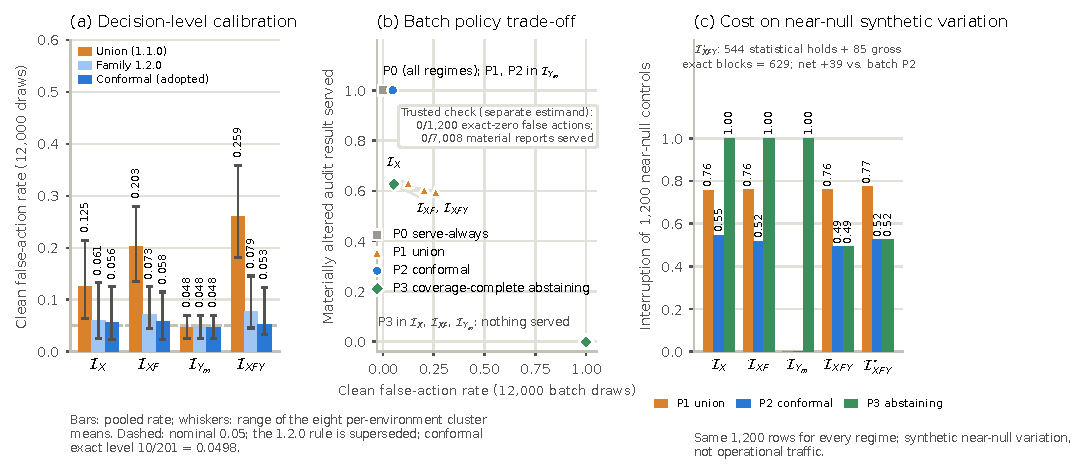
\includegraphics[width=\textwidth]{fig_q1_policy_decisions.pdf}
  \caption{Gates F and D (frozen evidence of artifact 1.3.0). (a)
  Decision-level false-alarm rate on \NEvalDraws{} disjoint clean draws of the
  union rule, of the superseded asymmetric rule and of the conformal family
  rule per regime; whiskers span the eight per-environment cluster means. (b)
  Unsafe-allow rate against clean false-action rate for every policy and
  regime at the primary materiality threshold; the trusted regime is the only
  point at the origin, its clean denominator is the 1,200 exact-zero rows,
  and the coverage-complete abstaining policy P3 serves nothing where the
  label boundary has no coverage. (c) Interruption of the same 1,200
  near-null synthetic controls by each policy and regime; the trusted
  regime's origin in (b) costs \BenignInterruptFamilyIXFYtrusted{} controls
  here, \BenignHoldFamilyIXFYtrusted{} statistical holds and
  \BenignBlockFamilyIXFYtrusted{} exact-reference blocks.}
  \label{fig:policy}
\end{figure*}

\subsection{Offline End-to-End Decisions}

Table~\ref{tab:policy} and Fig.~\ref{fig:policy}(b,c) report the offline
end-to-end evaluation. Under P0 every one of the \NMaterial{} material
observations is served. Under the batch-level regimes the conformal policy P2
serves \UnsafeFamilyIX{} ($\IX$), \UnsafeFamilyIXF{} ($\IXF$) and
\UnsafeFamilyIXFY{} ($\IXFY$) of them with clean false-action rates
\DecFprFamilyIX{}, \DecFprFamilyIXF{} and \DecFprFamilyIXFY{}, whereas the
uncalibrated union serves \UnsafeUnionIX{}, \UnsafeUnionIXF{} and
\UnsafeUnionIXFY{} at \DecFprUnionIX{}, \DecFprUnionIXF{} and
\DecFprUnionIXFY{}: the union buys \ContainUnionIXFY{} versus
\ContainFamilyIXFY{} containment in $\IXFY$ at more than four times the clean
false-action rate and \BenignHBUnionIXFY{} versus \BenignHBFamilyIXFY{}
interruption of the near-null controls. The earlier asymmetric rule served
\UnsafeLegacyFamilyIX{}, \UnsafeLegacyFamilyIXF{} and
\UnsafeLegacyFamilyIXFY{}; the correction moves the count by less than 1\% of
the material rows. The unsafe allows are dominated by structure, not by
thresholds: all \NMaterialLabel{} material label observations are served
under $\IX$ and $\IXF$ (residual blind region), \UnsafeFamilyLabelIXFY{} of
them under batch-level $\IXFY$ (statistically undetectable), and
\UnsafeFamilyDropoutIXF{} of \NMaterialFamDropout{} material dropout
observations under $\IXF$; $\IYm$ contains nothing in this suite.

The trusted-reference regime serves none of the \NMaterial{} material
observations with zero clean false actions on its 1,200 exact-zero rows (the
aggregate reference alone would suffice, by Corollary~3a), and blocks every
non-identity relabeling and every prediction change through its item-aligned
references. Its cost has two parts. Of the 1,200 near-null synthetic
controls the trusted calibrated policy interrupts
\BenignInterruptFamilyIXFYtrusted{}: \BenignHoldFamilyIXFYtrusted{} are
statistical holds by its batch-level component, the specificity cost of the
cluster fingerprint that P2 already pays in the batch regimes
(\BenignHoldFamilyIXFY{}--\BenignHoldFamilyIX{} holds), and
\BenignBlockFamilyIXFYtrusted{} are exact-reference blocks of controls whose
predictions changed under a 0.001 perturbation. Exact provenance therefore
adds \BenignBlockFamilyIXFYtrusted{} of 1,200 to a statistical cost the
calibrated batch-level policy incurs anyway; the total is
\BenignHBFamilyIXFYtrusted{} against \BenignHBFamilyIXF{} for P2 in $\IXF$
(Fig.~\ref{fig:policy}(c)). The controls are synthetic near-null variation,
not operational traffic, so neither number is a production false-positive
rate, and the two denominators of Table~\ref{tab:policy} are reported side by
side. The coverage-complete abstaining policy P3
makes information-set conditionality literal: in $\IX$, $\IXF$ and $\IYm$
the label boundary has no coverage, so nothing is served and every clean and
near-null row is interrupted; in $\IXFY$ and $\IXFYs$ every boundary is
covered and P3 coincides with P2, including P2's \UnsafeFamilyIXFY{} unsafe
allows in $\IXFY$: abstention on missing coverage is not a guarantee of
power, and the choice between P2 and P3 is a declared risk decision, not a
detector property. The composition with the six frozen contract envelopes
reproduces their actions (supplement).

\begin{table}[!t]
\caption{Offline decisions on frozen observations at the structural-sensitivity endpoint $|\Delta_R|>0$ (7,008 materially altered audit results among 10,800 interventions). P1: union; P2: conformal, risk-tolerant; P3: coverage-complete abstaining. FPR is estimated on 12,000 disjoint clean draws for batch regimes; the starred row instead reports an exact-zero invariant check on 1,200 rows and is not the same estimand. Benign is interruption of the same 1,200 near-null synthetic controls. Served: undetected materially altered audit results served, not malicious network events. Blind: structurally indistinguishable material rows.}
\label{tab:policy}
\centering
\scriptsize
\setlength{\tabcolsep}{2pt}
\begin{tabular}{@{}llrrrrr@{}}
\toprule
Regime & Policy & FPR/check & Benign & Served & Contain. & Blind \\
\midrule
$\mathcal I_X$ & P1 union & 0.125 & 0.76 & 4,429 & 0.37 & 2,617 \\
$\mathcal I_X$ & P2 conf. & 0.056 & 0.55 & 4,496 & 0.36 & 2,617 \\
$\mathcal I_X$ & P3 abst. & 1.000 & 1.00 & 0 & 1.00 & 2,617 \\
\addlinespace[1pt]
$\mathcal I_{XF}$ & P1 union & 0.203 & 0.76 & 4,231 & 0.40 & 2,617 \\
$\mathcal I_{XF}$ & P2 conf. & 0.058 & 0.52 & 4,365 & 0.38 & 2,617 \\
$\mathcal I_{XF}$ & P3 abst. & 1.000 & 1.00 & 0 & 1.00 & 2,617 \\
\addlinespace[1pt]
$\mathcal I_{Y_m}$ & P1 union & 0.048 & 0.00 & 7,008 & 0.00 & 5,450 \\
$\mathcal I_{Y_m}$ & P2 conf. & 0.048 & 0.00 & 7,008 & 0.00 & 5,450 \\
$\mathcal I_{Y_m}$ & P3 abst. & 1.000 & 1.00 & 0 & 1.00 & 5,450 \\
\addlinespace[1pt]
$\mathcal I_{XFY}$ & P1 union & 0.259 & 0.76 & 4,180 & 0.40 & 0 \\
$\mathcal I_{XFY}$ & P2 conf. & 0.053 & 0.49 & 4,390 & 0.37 & 0 \\
\addlinespace[1pt]
$\mathcal I_{XFY}^{\star}$ & P2/P3 (exact) & 0.000 & 0.52 & 0 & 1.00 & 0 \\
\bottomrule
\end{tabular}
\end{table}


\subsection{Adaptive Cluster-Preserving Attacker}

Gate~A ran as preregistered: 240 of 240 jobs, and the clean rows and matched
controls reproduce the frozen expansion rows exactly. The attacker perturbs
\AdvPerturbedMean{} of the entries on average
(\AdvPerturbedMin{}--\AdvPerturbedMax{} across environments, branches and
dimensions); Fig.~\ref{fig:adversarial} and the supplement report the
outcome. At the matched strengths 0.02, 0.05 and 0.10 the conformal rule
detects the executed mean shift in \AdvDetCtrlMSTwoPctIX{},
\AdvDetCtrlMSFivePctIX{} and \AdvDetCtrlMSTenPctIX{} of the rows in $\IX$ and
its cluster-preserving variant in \AdvDetAdaptMSTwoPctIX{},
\AdvDetAdaptMSFivePctIX{} and \AdvDetAdaptMSTenPctIX{}
(\AdvDetAdaptMSTwoPctIXF{}, \AdvDetAdaptMSFivePctIXF{} and
\AdvDetAdaptMSTenPctIXF{} in $\IXF$); scaling drift behaves alike
(\AdvDetAdaptSDTwoPctIX{}--\AdvDetAdaptSDTenPctIX{} in $\IX$ against
\AdvDetCtrlSDTwoPctIX{}--1.00). The attacker keeps most of the harm: the
material fraction of the cluster-preserving mean shift is
\AdvMatAdaptMSTwoPct{}, \AdvMatAdaptMSFivePct{} and \AdvMatAdaptMSTenPct{}
against \AdvMatCtrlMSTwoPct{}, \AdvMatCtrlMSFivePct{} and
\AdvMatCtrlMSTenPct{}. Detection recovers at 0.25 and 0.50, where the
unclustered entries move far enough to shift the feature distribution against
the between-batch null. The classical branch (standardized features) is more
evasive than the quantum branch (features scaled to $[0,2\pi]$): at strength
0.10 the mean shift is detected in \AdvDetClassicalMSTenPctIX{} and
\AdvDetClassicalMSTenPctIXF{} of classical cells and
\AdvDetQuantumMSTenPctIX{} and \AdvDetQuantumMSTenPctIXF{} of quantum cells
in $\IX$ and $\IXF$, with the same cluster rule; the scaler sets how far the
unclustered entries move. Of the \AdvNMaterialAdaptIXF{} material
adaptive rows, P2 serves \AdvUnsafeAdaptFamilyIX{} in $\IX$,
\AdvUnsafeAdaptFamilyIXF{} in $\IXF$ and \AdvUnsafeAdaptFamilyIXFY{} in
$\IXFY$, against \AdvUnsafeCtrlFamilyIX{}, \AdvUnsafeCtrlFamilyIXF{} and
\AdvUnsafeCtrlFamilyIXFY{} of \AdvNMaterialCtrlIXF{} for the executed
mechanisms in the same runs; under $\IXFYs$ every material adaptive row is
blocked, because a changed conclusion with fixed labels requires a changed
prediction. The ``detected in every cell'' result for feature drift was a
property of the fingerprint, not of the mechanism: calibration controls false
alarms but buys no coverage against an attacker who knows what the sensor
sees; only a reference does.

\begin{figure}[!t]
  \centering
  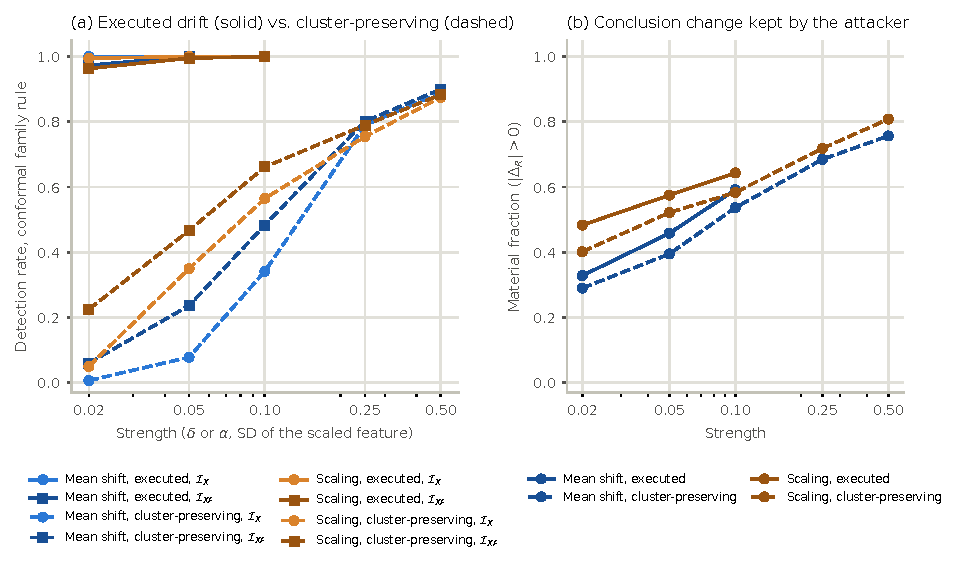
\includegraphics[width=\columnwidth]{fig_q1_adversarial_cluster_preserving.pdf}
  \caption{Gate~A. (a) Detection under the conformal family rule of the
  executed drift mechanisms (solid) and of their cluster-preserving variants
  (dashed) in $\IX$ and $\IXF$, 600 observations per point. (b) Material
  fraction of the same rows: the attacker evades the batch-level sensors at
  matched strengths while keeping most of the conclusion changes.}
  \label{fig:adversarial}
\end{figure}

\subsection{Quantum-Workflow Coverage}

All 165 cells are present and all nine prespecified acceptance checks pass;
the supplement tabulates and plots the response fraction of every sensor per
condition, read class by class. In this ideal-statevector gate the honest
estimate equals the semantic kernel and $g$ is the identity, so one anchored
comparison against $\Phi(C_0)$ serves as the semantic probe on circuit-side
rows and as the observed-kernel reference on post-processing rows; under
finite-shot estimation the two anchors separate (Proposition~7(iii)). Clean
cells trigger no sensor. Benign transpilation and the common-unitary rewrite
change serialized provenance while preserving semantic kernels, algebraic
properties and outputs in every cell (Proposition~7(i)): a raw hash
difference needs policy-aware adjudication. Every data-dependent circuit
mutation changes the semantic kernel; the mild RZ mutation changes no
prediction, the stronger one changes predictions in 2/15 cells and the
repetition change in 11/15. Asymmetric and diagonal-eroded matrices are
detected algebraically in every cell and change no prediction; the
PSD-preserving mixture is symmetric, unit-diagonal and PSD in all cells, so
algebraic validation is exactly blind, the circuit hash sees nothing because
$C$ is unchanged, and only the kernel hash and the anchored comparison of the
observed kernel expose all 15 substitutions, with output monitoring reacting
in 1/15 (Proposition~7(ii)). Both shot emulators produce non-zero
repeated-estimation discrepancy in all 30 cells and output changes in 7/15
and 3/15, a property of these cells rather than the universal law that
Proposition~7(iii) declines to state; the contract holds them for
adjudication instead of testing exact equality. The prototype's six envelopes
verify and its eight acceptance checks pass (clean and approved transpilation
allowed; parameterized mutation and PSD-preserving substitution blocked;
prior-preserving label corruption blocked at the evaluation contract despite
a zero class-prior delta; the approved 256-shot emulator held). The secondary
ZZ-versus-SVC comparison (supplement) is retained only to show that the
primary result does not depend on the model: its direction is stable, its
magnitude conditional on scalers and clean headroom, and it is neither a
quantum-advantage nor a vulnerability ordering.

\section{Integrity-Audit Contract}

The evidence yields a reporting and enforcement contract: every integrity
claim names the boundary and protected asset, the adversary or failure class
and what remains fixed, the information regime and trusted references it
assumes, the sensor, the calibration rule and its decision-level level with
its premise, the covered interventions, the structural, calibrated and
adaptive residual blind regions, the cost on near-null variation, and the
response. For the label path the minimum bundle is item-level label
provenance plus a joint label-prediction audit; for the studied quantum
boundary it is authenticated circuit/parameter provenance, an
approved-transpilation policy, semantic probe kernels, a reference on the
observed kernel, algebraic checks, repeated-estimation evidence and
abstention where no null is calibrated. The contracts fail closed on their
invariants (a violated invariant blocks, missing mandatory evidence holds);
P2 may serve under an explicitly declared residual blind region; P3 abstains
whenever a mandatory boundary lacks declared exact or statistical coverage and
makes no promise about the power of the coverage that exists. Neither
converts missing evidence into a claim of integrity; P2 converts it into a
declared, accepted risk.

\section{Discussion and Limitations}

\subsection{Security Interpretation}

A metric can move while predictor output is bit-for-bit unchanged, and it can
move upward; calling either model degradation assigns failure to the wrong
component and suggests the wrong defence, since input robustness cannot
repair corrupted ground truth while provenance and joint validation can. Zero
sensor response is informative only if the sensor receives evidence capable
of distinguishing the states, and non-zero separability only if the auditor
holds a null tight enough to see it. The offline end-to-end result makes the
consequence concrete: with the evidence a batch-level auditor normally has,
about three fifths of the materially changed results in this suite would be
served under a calibrated policy, and the share is set by the information
regime, not by the threshold. The adversarial gate adds the second half of
the lesson: a calibrated sensor family controls false alarms but not what an
adaptive attacker can hide from it, so the ``fully detected'' mechanisms of
the frozen suite are served in 28--39\% of their material instances once the
attacker preserves the fingerprint. The lever is provenance, whose
granularity follows the integrity notion: a trusted aggregate of the same
batch certifies the conclusion, item alignment certifies item identity, and
nothing the adversary can rewrite certifies anything (Proposition~6). Its
price is measured rather than hidden and is mostly statistical: the trusted
policy interrupts \BenignInterruptFamilyIXFYtrusted{} of 1,200 near-null
synthetic controls, \BenignHoldFamilyIXFYtrusted{} statistical holds that the
calibrated batch-level policy pays as well and \BenignBlockFamilyIXFYtrusted{}
exact-reference blocks that the same-batch anchor adds.

\subsection{Validity Boundaries}

Three datasets and eight fixed scale/temporal settings, six of the nine
environments from CICIDS2017, are not sampled deployments; five split
clusters measure within-environment resampling only; most gates use 128/128
samples; balanced numeric-only staging does not reproduce operational
prevalence. Both quantum evaluators are ideal statevector simulators with
binomial shot emulation. SVC and QSVC keep pipeline-specific scalers, so their
comparison does not isolate kernel geometry, and the same scalers govern how
far an adaptive attacker's unclustered entries move. Exact blindness is a
capability result under constructed perturbations and estimates no
prevalence. The conformal level is marginal and holds under exchangeability
of the calibration draws and the audited batch; the executed design violates
that premise (draws overlap within a pool half, the calibration and
evaluation halves are different rows of one table, and E1's pool half
supplies one disjoint batch), the residual excess is reported as executed,
and no conditional guarantee given a calibration set is claimed. The
adversarial gate fixes one cluster rule and two mechanisms; an attacker with
a different model of the sensors is not evaluated. The trusted item-aligned
regime is a trust assumption, not a stronger detector: if the reference can
be rewritten with the asset, Proposition~6 applies, and its interruption cost
is measured on near-null synthetic controls, not on operational traffic. P3
abstains on missing coverage only; a boundary nominally covered by a
low-power sensor remains a limitation of every policy here, and abstention
conditioned on the validity of the calibration itself is not part of this
layer. The prototype is a local process without authenticated provider
records, and its hash chain certifies consistency of the record, not its
authenticity. Every policy result is offline, on frozen outputs.
Context-conditioned runtime calibration under non-stationarity,
out-of-support abstention with recovery, real-QPU execution and the
service-level evaluation of enforcement are the subject of a separate study.

\section{Conclusion}

Hybrid workflow integrity cannot be reduced to a robustness number. An
intervention can change a reported conclusion without changing the model, a
sensor can stay silent because its view is identical, a separable change can
stay undetected because the auditor holds no same-batch anchor, and a
detected change can become undetected once the attacker learns what the
sensor sees. We formalized this as observational indistinguishability under
explicit information sets and trusted references, derived monotone and
exactly closable blind regions with the label path as a protected boundary,
placed the quantum branch on the same lattice, confirmed the boundaries
across three datasets and eight environments, calibrated the decision with a
conformal rule whose finite-sample level holds under exchangeability and
whose observed rates in the executed design are reported as such, and
measured offline what each regime serves, what it costs on near-null
variation and how an adaptive attacker evades it. Every integrity claim must
therefore state its boundary, view, trusted roots, decision-level level and
premise, residual and adaptive blind regions, cost and response; assurance is
granted only when the evidence the claim requires is present.

\section*{Data, Code, and Ethics Statement}

The review artifact contains source code, a locked environment, tests, compact
derived tables, figures, seven SHA-256 evidence manifests, reproduction
commands, the preregistrations of the 1.1.0--1.3.0 gates and the amendment
that replaced the calibration rule. Raw CICIDS2017, UNSW-NB15 and ToN-IoT
data are not redistributed; their sources, expected hashes and deterministic
staging are documented. The experimental evidence is frozen at artifact 1.3.0
(version DOI 10.5281/zenodo.22648573). Version
1.3.1 is archived at Zenodo under the concept DOI 10.5281/zenodo.22550852
(version DOI in the artifact metadata); code is released under Apache-2.0,
derived evidence, figures and documentation under CC~BY~4.0. The study uses
previously released benchmarks and involves no new human-participant or
personal-data collection.

\section*{Acknowledgment}

During manuscript and artifact preparation the authors used two generative-AI
coding assistants. OpenAI Codex (May--August 2026) assisted with literature
discovery, drafting and language editing of the manuscript, code inspection,
and the evidence builders, verifier and tests of artifact 1.0.0. Anthropic
Claude Code (September 2026) assisted with the related-work additions, the
formal section and its counterexamples, the adversary model, text edits
throughout the article and supplement, the artifact 1.1.0--1.3.1 code
(samplers, queues, evidence builders, policy layer, conformal rule and its
tests, adversarial gate, generators, assembler, release automation), the
mathematical audit that found the defect in the earlier calibration rule and
the formal and editorial corrections of version 1.3.1. The authors specified
the protocols, verified the primary sources, proofs, numerical results, code
and generated text, and retain full responsibility for the article.

% Column balance of the last page: set \IEEEtriggeratref{N} only if the reference list ends unbalanced.
\bibliographystyle{IEEEtran}
{\sloppy\bibliography{references}}

\end{document}
